%% MoCHII code paper -- draft.
%% AASTeX v7.0.2.  Target journal: ApJ / ApJS.
%% Author: Kwang-Il Seon (KASI / UST).
%%
%% Build: pdflatex mochii ; bibtex mochii ; pdflatex mochii ; pdflatex mochii
%%
%% Numerical values, validation results, and equations are taken from the project
%% development record (../CLAUDE.md) and the physics memo
%% (../docs/MoCHII_physics.tex).  Do not alter numbers without checking those
%% sources.

\documentclass[twocolumn,linenumbers]{aastex702}

\usepackage{amsmath}
\usepackage{amssymb}
\usepackage{booktabs}
\usepackage{array}

%% ---- convenience macros ----
\newcommand{\code}[1]{\texttt{#1}}
\newcommand{\MoCHII}{\textsc{MoCHII}}
\newcommand{\MoCafe}{\textsc{MoCafe}}
\newcommand{\Mthree}{M$^{3}$}
\newcommand{\HII}{H\,\textsc{ii}}
\newcommand{\HI}{H\,\textsc{i}}
\newcommand{\HeI}{He\,\textsc{i}}
\newcommand{\HeII}{He\,\textsc{ii}}
\newcommand{\HeIII}{He\,\textsc{iii}}
\newcommand{\Te}{T_{\mathrm{e}}}
\newcommand{\nelec}{n_{\mathrm{e}}}
\newcommand{\nH}{n_{\mathrm{H}}}
\newcommand{\xHI}{x_{\mathrm{HI}}}
\newcommand{\QH}{Q_{\mathrm{H}}}
\newcommand{\cmc}{\mathrm{cm^{3}\,s^{-1}}}

\shorttitle{MoCHII: Monte Carlo photoionization on octree AMR}
\shortauthors{Seon}

\begin{document}

\title{MoCHII: A Three-Dimensional Monte Carlo Photoionization
Code for Dusty Nebulae on Adaptive Octree Grids}

%% TODO: confirm final title.
\author[orcid=0000-0001-9561-8134,gname=Kwang-Il,sname=Seon]{Kwang-Il Seon}
\affiliation{Korea Astronomy and Space Science Institute,
776 Daedeokdae-ro, Yuseong-gu, Daejeon 34055, Republic of Korea}
\affiliation{Department of Astronomy and Space Science,
University of Science and Technology, Korea,
217 Gajeong-ro, Yuseong-gu, Daejeon 34113, Republic of Korea}
\email[show]{kiseon@kasi.re.kr}

\begin{abstract}
We present \MoCHII{} (MOnte Carlo for \HII{} regions), a
three-dimensional Monte Carlo radiative-transfer code for dusty
photoionized nebulae on adaptive octree (AMR) grids.  \MoCHII{} is built
by adding a self-consistent gas-physics layer to the validated octree
transport, peel-off, and stochastic-dust modules of the dust code
\MoCafe{}, and it computes hydrogen and helium photoionization and
thermal balance, a trace-metal ionization cascade with modern analytic
atomic data, the dust and PAH continuum, and the recombination-line and
nebular-continuum diagnostics all from one radiation field.  The band
transport uses an analytic (zero-variance) direct-field estimator on the
octree together with a dedicated Cartesian digital-differential-analyzer
(DDA) backend, an explicit Monte Carlo diffuse field, dust absorption and
forward scattering, and observer peel-off imaging.  The atomic data are
fitted offline and evaluated online: exact hydrogenic \HI/\HeII{} cross
sections, Verner et al.\ (1996) fits for the remaining ions, Badnell
(2023) radiative and dielectronic recombination with the case A/B
ground-level split taken from the Milne relation on those same cross
sections, Voronov collisional ionization,
and charge exchange, so that adding a metal ion is a data operation
rather than a code operation.  We validate the code against analytic
attenuation (rate-integral bias $+0.08\%$), the Str\"omgren sphere
(ionized volume $+0.68\%$ versus an exact 1D reference; AMR identical to
a uniform grid), a thermal H/He nebula (median $0.77\%$ in $\Te$), and
the Lexington 2000 \HII{} region benchmarks.  Its line cooling is taken
from the level populations at the local electron density, the same
$n$-level solve that produces the emergent lines, so the thermal balance
and the line list are one physics.  On the two benchmarks the
$n_{\mathrm{p}}n_{\mathrm{e}}$-weighted temperature then agrees with a
\textsc{Cloudy} c25.00 calculation of the same models to $0.5\%$ (HII40)
and $0.2\%$ (HII20), with the He$^{+}$/H$^{+}$ ratio and the outer radius
inside the published multi-code ranges; the cooling itself is
cross-validated channel by channel against a \textsc{Cloudy} c25.00
decomposition on a fixed $(\Te, \nelec, \mathrm{ionization})$ state, where
it agrees to $1\%$.  We further demonstrate
solution-driven ionization-front re-refinement (a re-refined octree
reproduces a native high-resolution grid to $+0.008\%$ in ionized volume
with $4.5\times$ fewer cells), the complete dust and PAH coupling (grain
heating energy closure $L_{\mathrm{IR}}/L_{\mathrm{abs}} = 1.000$; the
projected 8\,$\mu$m image turning from a central peak into a
limb-brightened ionization-front annulus as PAHs are destroyed in ionized
gas), and an atomic photodissociation-region
skin with photoelectric heating.  \MoCHII{} is written for modern
three-dimensional synthetic observations of \HII{} regions and their
surroundings.
\end{abstract}

\keywords{\uat{H II regions}{694} --- \uat{Interstellar medium}{847}
--- \uat{Radiative transfer}{1335} --- \uat{Photoionization}{2060}
--- \uat{Interstellar dust}{836} --- \uat{Astronomy software}{1855}}

%==========================================================================
\section{Introduction}
\label{sec:intro}

Photoionized regions --- \HII{} regions, planetary nebulae, the diffuse
ionized medium, and the circumgalactic gas illuminated by stars and
active nuclei --- are among the most information-rich objects in
astrophysics.  Their emission-line and continuum spectra encode the
ionizing radiation field, the elemental abundances, the electron
temperature and density, and the dust content of the gas.  Extracting
that information requires a radiative-transfer model that couples the
ionizing radiation field to the ionization, thermal, and dust state of
the gas self-consistently.

The classic tools for this problem are one-dimensional: \textsc{Cloudy}
\citep{cloudy2017,cloudy2023} and \textsc{Mappings}
\citep{sutherland1993,mappingsv2017} solve the coupled ionization,
thermal, and (in the case of \textsc{Mappings}) shock structure of a
spherical or plane-parallel slab with very detailed microphysics: large
ion inventories, density-dependent multilevel cooling, non-equilibrium
and time-dependent options, and grain and PAH physics.  Their strength is
completeness of the local physics; their limitation is geometry.  Real
\HII{} regions are clumpy, aspherical, and shadowed, and the diffuse
recombination field they produce is intrinsically three-dimensional.

Three-dimensional Monte Carlo photoionization codes were developed to
address exactly this geometry.  \textsc{Mocassin}
\citep{ercolano2003,ercolano2005,ercolano2008} pioneered the
self-consistent Monte Carlo treatment of the direct and diffuse fields on
a Cartesian grid, with a large ion and dust inventory, and it defines the
\emph{de facto} three-dimensional benchmark suite (the Lexington/Meudon
comparison cases; \citealt{ferland1995,pequignot2001}).  The code of
\citet{wood2004} demonstrated Monte Carlo photoionization with an
efficient path-length estimator for the mean intensity.  \textsc{M}$^{3}$
(Messenger Monte Carlo \textsc{Mappings V}; \citealt{jin2022,jin2022fractal})
grafts three-dimensional Monte Carlo transport onto the extensive
\textsc{Mappings V} microphysics, combining broad atomic physics with
arbitrary Cartesian geometry.  \textsc{CMacIonize}
\citep{cmacionize2018} adds a task-based, unstructured (Voronoi or
adaptive Cartesian) grid and a modern software design.  These codes
share a common architectural constraint: their spatial grids are either
uniform Cartesian or, in the \textsc{CMacIonize} case, unstructured, and
their diffuse-field and grid-traversal designs are tightly coupled.

\MoCHII{} (MOnte Carlo for \HII{}
regions)\footnote{\url{https://github.com/seoncafe/MoCHII}} is a new
three-dimensional
Monte Carlo photoionization code built around a different design choice:
it reuses the mature octree adaptive-mesh-refinement (AMR) engine,
event-driven traversal, peel-off imaging, and stochastic dust/PAH
emission of the dust radiative-transfer code \MoCafe{} (Seon, in
preparation)\footnote{\url{https://github.com/seoncafe/MoCafe}}, and
adds a gas-physics layer on top.  The motivation is
practical.  Retrofitting an octree traversal onto an existing uniform-grid
photoionization code is difficult: the ray-segment bookkeeping is
entangled with the physics loop, and structural rewrites are error-prone
(the \textsc{Mocassin} \code{pathSegment} traversal, for instance,
carries a dual position representation with many mutation sites).  An
event-driven AMR transport engine, by contrast, already \emph{is} the
design such a retrofit would have to reach.  \MoCafe{} provides that
engine, validated for dust transport, so \MoCHII{} inherits octree AMR,
an analytic direct-field estimator, a dedicated Cartesian
digital-differential-analyzer (DDA) backend, peel-off synthetic imaging,
MPI-3 shared-memory parallelism, and HDF5/FITS I/O without modifying the
dust tree.

On top of that engine \MoCHII{} adds: (i) a continuous-energy ionizing
photon sampler, with a grouped threshold-aligned compatibility mode, and a
zero-variance direct-field estimator;
(ii) hydrogen and helium photoionization and thermal balance with modern
recombination data; (iii) a trace-metal ionization cascade organized as a
data-driven registry, so that adding an ion (currently eleven elements,
C through Ca) is an offline data operation; (iv) an explicit Monte Carlo
diffuse field with a case-A/B option; (v) the complete dust and PAH
coupling in the ionizing and far-ultraviolet (FUV) bands, including
equilibrium and stochastic dust emission; (vi) solution-driven
ionization-front re-refinement of the octree; and (vii) recombination-line,
collisional-line, and nebular-continuum diagnostics with leaf-resolved
emissivity output for synthetic imaging.  The atomic data are fitted
offline from CHIANTI and the Strathclyde/Badnell tables and evaluated by
analytic formulae at run time, with a provenance header on every
coefficient file.

The remainder of this paper is organized as follows.
Section~\ref{sec:compare} compares \MoCHII{} with the established 1D and
3D codes.  Section~\ref{sec:methods} describes the Monte Carlo transport,
the grids, the diffuse field, the iteration and convergence scheme, and
the quasi-random launch option.  Section~\ref{sec:atomic} documents the
atomic data and the offline fitting pipeline.
Section~\ref{sec:validation} presents the validation against analytic
solutions and the Lexington benchmarks.
Section~\ref{sec:refine} demonstrates the solution-driven I-front
re-refinement and a cosmological post-processing application.
Section~\ref{sec:dust} presents the dust and PAH coupling, and
Section~\ref{sec:pdr} the photodissociation-region skin.
Section~\ref{sec:summary} summarizes and outlines planned extensions.

%==========================================================================
\section{Comparison with existing codes}
\label{sec:compare}

Table~\ref{tab:compare} places \MoCHII{} next to the reference codes along
the axes most relevant to three-dimensional nebular modeling.  The
comparison is deliberately architectural rather than a claim of superior
physics: \textsc{Cloudy} and \textsc{Mappings} carry more complete local
microphysics (larger ion inventories, full multilevel cooling of every ion,
non-equilibrium and shock options), and \textsc{Mocassin} carries a
comparably broad ion and dust inventory in three dimensions.  \MoCHII{}'s
distinguishing features are the octree AMR grid with solution-driven
re-refinement, the reuse of a validated dust-transport engine (so that
dust absorption, forward scattering, equilibrium and stochastic emission,
and PAH physics are first-class rather than bolted on), and the
peel-off synthetic-imaging output.

The grid axis is the sharpest distinction.  \textsc{Mocassin} and
\textsc{M}$^{3}$ use uniform Cartesian grids; \textsc{CMacIonize} uses an
unstructured Voronoi or adaptive Cartesian grid; \MoCHII{} uses an octree
whose refinement can be driven by the ionization solution itself
(Section~\ref{sec:refine}).  On the Str\"omgren problem this lets
\MoCHII{} concentrate resolution at the ionization front and reproduce a
native high-resolution run with several times fewer cells.

The diffuse-field axis separates the on-the-spot (OTS) approximation from
explicit transport.  \MoCHII{} defaults to case-B OTS (no diffuse packets,
consistent with the analytic direct-field estimator) but offers an
explicit Monte Carlo diffuse field with case-A rates and
ground-recombination emission, matching the \textsc{Mocassin} and
\textsc{Cloudy} treatment; the benchmark runs of Section~\ref{sec:hii} use
it, so that the transfer treatment is the same on both sides of that
comparison.

The atomic-data axis reflects vintage.  \MoCHII{} uses exact hydrogenic
cross sections, Verner et al.\ (1996) fits, Badnell (2023) recombination,
CHIANTI v11 collision strengths, and a ground-level recombination
coefficient obtained from those cross sections through the Milne relation
--- the same modern data, and the same construction of the case A/B split,
that \textsc{Cloudy} uses --- rather than the older compilations still
carried by \textsc{Mocassin}.

The metal-treatment axis is easy to state wrongly, so we state it from the
distributed sources.  It is tempting to say that the established codes solve
one coupled nonlinear system over every element while \MoCHII{} treats the
metals as a perturbation.  That is not what the codes do.  None of
\textsc{Mocassin}, \textsc{CMacIonize}, \textsc{Torus}, the code of
\citet{wood2004}, or even \textsc{Cloudy} assembles the elements into a joint
system; all five advance one element at a time inside nested outer
iterations, with $T$ an outer root find in every case.  Four of the five use
the same nearest-neighbor ratio chain \MoCHII{} uses, adjacent-stage ratios
$f_{i+1}/f_i$ chained and normalized.  \textsc{Cloudy} does build a matrix,
but one per element, and needs it because Auger ejection jumps several stages
at once, which no adjacent-stage chain can represent.  The ratio chain is
therefore the standard method of the field rather than a \MoCHII{}
approximation, and these codes differ not in how the stage populations are
obtained but in which feedbacks are wired in.

On that axis \MoCHII{} is ahead of three of the four Monte Carlo codes.  It
attenuates the ionizing field with the metal photoionization opacity
(\code{ion\_metal\_abs}), where \textsc{CMacIonize}, \textsc{Torus}, and
\citet{wood2004} accumulate metal photoionization rates while never removing
those photons from the beam, so that a metal photoionization costs the
radiation field nothing.  That is not a small choice: switching the opacity
off moves $r(\mathrm{He}^{0}\!=\!0.5)$ inward by 0.615~pc at HII40, because
the stages with thresholds between 21 and 40~eV preferentially remove the
softest helium-ionizing photons while $\sigma(\HeI)/\sigma(\HI)$ rises from
6.1 at 25~eV to 19.9 at 95~eV, so the hardened surviving field is taken up by
$\mathrm{He}^{0}$ rather than $\mathrm{H}^{0}$.  \MoCHII{} also solves the
metal contribution to $\nelec$ as a fixed point rather than a single
evaluation (\code{metal\_ne}), since the stage fractions depend on $\nelec$
themselves and one evaluation at the H/He-only electron density is the
$\nelec \to 0$ limit in which nothing recombines; \textsc{CMacIonize} and
\citet{wood2004} count no metal electrons at all.  \code{metal\_heat} adds
metal photoheating, which \textsc{Mocassin} includes and those two omit.
Both now default on, the measurement in
Section~\ref{sec:cooldata} having settled what leaving them off costs; the
benchmark runs of Section~\ref{sec:hii} enable them explicitly, so every metal
feedback \MoCHII{} implements is active in those numbers.  The trace
separation describes the solution method, not a switched-off feedback.

One feedback the other four Monte Carlo codes also omit is charge exchange
being two-way in the bookkeeping:
$\mathrm{X}^{i+} + \mathrm{H}^{+} \to \mathrm{X}^{(i+1)+} + \mathrm{H}^{0}$
recombines the metal and ionizes hydrogen in the same event, so it is a source
and a sink on both sides, and \textsc{Cloudy} alone puts hydrogen's side into
hydrogen's own balance.  \MoCHII{} now does too
(\code{par\%charge\_exchange}, the default); a fixed-state gate holds all 29
reactions to $6.5\times10^{-16}$ between the two sides.  The correction is
small here for a structural reason: where the near-resonant
$\mathrm{O}^{0}/\mathrm{H}^{+}$ pair locks oxygen to hydrogen, the two terms
cancel identically in hydrogen's balance, so what survives is the departure
from that lock.  Measured,
$\langle T[N_{\mathrm{p}}N_{\mathrm{e}}]\rangle$ moves $-1.4$~K at HII40 and
$-0.1$~K at HII20, and every front by under $0.001$~pc --- 58 and 533 times
inside the tolerance these runs were converged to, so
Tables~\ref{tab:wood40} and~\ref{tab:wood20} are not re-baselined on them.
The same near-cancellation dictates how the balance is solved: it leaves the
substitution map marginally stable in partially neutral gas, so \MoCHII{}
solves hydrogen's balance for its root rather than substituting into it, with
the cascade re-evaluated at each trial.  The root is bracketed in $[0,1]$ by
construction, so the fraction cannot leave the physical range; one cell solve
converges to $4\times10^{-11}$ where substitution left $2\times10^{-3}$, and
the residual beyond the front falls three orders of magnitude while
$\langle T[N_{\mathrm{p}}N_{\mathrm{e}}]\rangle$ moves 0.01~K.  The one
remaining absence is metal recombination continua as a diffuse source, worth
0.29\% of the explicit diffuse channel that dominates the helium budget; it
and the measurements that size it are planned in
\code{docs/METAL\_COUPLING\_PLAN.md}, and the full source-level comparison is
in \code{docs/MoCHII\_code\_comparison.tex}.  What the registry buys is
unchanged: adding an ion remains a data-file addition rather than a change to
a coupled solver (Section~\ref{sec:atomic}).

A related but separate axis is the cooling inventory --- which channels a
code carries at all, since that is what sets the equilibrium temperature.
As implemented in the distributed source, the Monte Carlo code of
\citet{wood2004} cools by ten five-level metal ions (N\,\textsc{i},
N\,\textsc{ii}, O\,\textsc{i}, O\,\textsc{ii}, O\,\textsc{iii},
Ne\,\textsc{iii}, S\,\textsc{ii}, S\,\textsc{iii}, C\,\textsc{ii},
C\,\textsc{iii}) plus two two-level ions ([N\,\textsc{iii}]
57\,$\mu$m and [Ne\,\textsc{ii}] 12.8\,$\mu$m), and \textsc{CMacIonize} by
the same ten five-level ions plus three two-level ions, adding
[S\,\textsc{iv}] 10.5\,$\mu$m; both then add free-free emission and
hydrogen and helium recombination cooling, in each case with the H$^{+}$
and He$^{+}$ terms only.  \MoCHII{}
carries line cooling for 28 ions --- \HI{} and the 27 metal ions of the
eleven-element registry (Appendix~\ref{app:atomic}) --- and adds three
channels that neither of those two codes carries: \HI{} collisional
excitation, collisional-ionization cooling of H and He, and the He$^{++}$
terms of the free-free and recombination sums.  In a $10^4$~K \HII{}
region these are small (\HI{} collisional lines are $0.7\%$ of the
HII40 cooling budget), but they are the terms that take over in the hot,
partly neutral gas of an ionization front and in the shielded gas beyond
it.

\begin{deluxetable*}{>{\raggedright\arraybackslash}p{2.4cm}>{\raggedright\arraybackslash}p{2.5cm}>{\raggedright\arraybackslash}p{2.3cm}>{\raggedright\arraybackslash}p{2.3cm}>{\raggedright\arraybackslash}p{2.3cm}>{\raggedright\arraybackslash}p{2.3cm}}
\tablecaption{Architectural comparison of \MoCHII{} with reference
photoionization codes.  ``OTS'' = on-the-spot (case B); ``explicit'' =
transported diffuse field.  This table compares design, not the breadth
of local microphysics, on which the 1D codes and \textsc{Mocassin} are
more complete.  The two metal rows are read from the distributed sources
for \MoCHII{}, \textsc{Mocassin}, \textsc{CMacIonize}, and \textsc{Cloudy};
the \textsc{M}$^{3}$ entries follow its documentation.\label{tab:compare}}
\tablewidth{0pt}
\tabletypesize{\footnotesize}
\tablehead{\colhead{} & \colhead{\MoCHII{}} & \colhead{MOCASSIN} &
\colhead{M$^{3}$} & \colhead{CMacIonize} & \colhead{Cloudy / MAPPINGS}}
\startdata
Dimensionality & 3D & 3D & 3D & 3D & 1D \\[2pt]
Grid & octree AMR + Cartesian DDA & uniform Cartesian & uniform Cartesian & Voronoi / adaptive Cartesian & spherical / plane-parallel \\[2pt]
Solution-driven refinement & yes (I-front) & no & no & static AMR & 1D shells \\[2pt]
Diffuse field & OTS default; explicit MC option & explicit MC & explicit MC & explicit MC & outward-only / OTS \\[2pt]
Recombination data & Badnell 2023 + Milne $\alpha_1$ & Verner \& Ferland 1996 & MAPPINGS V & Verner / Badnell & Badnell / internal \\[2pt]
Metal ionization solve & ratio chain, one element at a time & ratio chain, one element at a time & MAPPINGS network & ratio chain, one element at a time & matrix, one element at a time (\textsc{Cloudy}) \\[2pt]
Metal feedbacks wired in & opacity, $\nelec$, photoheating, free-free, line cooling & opacity, $\nelec$, photoheating, line cooling & MAPPINGS set & line cooling only & all, plus two-way charge exchange \\[2pt]
Dust / PAH & absorption + forward scattering + equilibrium + stochastic + PAH survival & absorption + emission & MAPPINGS grains & absorption + emission & detailed grains/PAH \\[2pt]
Parallelism & MPI-3 shared memory & MPI & MPI & task-based / MPI & OpenMP / serial \\[2pt]
Synthetic output & peel-off images, line maps, IR SED & line maps, images & line maps & line maps, images & 1D spectra \\
\enddata
\end{deluxetable*}

%==========================================================================
\section{Methods}
\label{sec:methods}

\MoCHII{} follows the conventions of its parent dust code: all input is a
single Fortran namelist (\code{par}); computation is in double precision;
parallelism is MPI-only with MPI-3 shared-memory windows for the grid;
output is HDF5 with a FITS fallback; and algorithm variants are selected
by procedure pointers at startup.  A run reads (or builds) a grid, persists
a gas leaf state, and iterates transport and equilibrium to convergence.

\subsection{The ionizing band and the source}
\label{sec:band}

The ionizing band spans photon energies $[E_{\min}, E_{\max}] =
[13.598, 100]$~eV.  In continuous mode, the source spectrum --- a Planck
function $B_\nu(T_\star)$ or a tabulated spectrum in shape or physical
(per-eV, per-Hz, per-\AA, per-$\mu$m) units --- defines an energy-luminosity
probability density.  A packet energy is drawn by inversion of its CDF and
the photoionization cross sections and excess energy are evaluated at that
drawn energy.  Thus the $n_\nu$ bins (typically 32) are a diagnostic tally
of $J_E$, not a transport discretization; changing their count cannot change
the physical solution.  Packets carry $L_{\mathrm{pkt}} =
L_{\mathrm{band}}/N$.

\paragraph{Grouped mode.}  The grouped mode
(\code{ion\_energy\_mode = 'grouped'}) samples a bin from the luminosity CDF
and uses its representative energy.  In that mode, by default
(\code{ion\_align\_edges})
the bin \emph{edges} are pinned onto the ionization thresholds --- \HI{}
(13.6~eV), \HeI{} (24.6~eV), \HeII{} (54.4~eV), and the active metal
edges gathered from the registry --- so that no bin straddles a threshold;
the sub-segments between thresholds are log-uniform.  This removes a real
discretization error: a coarse 32-bin log grid straddles the 24.6~eV \HeI{}
edge and delivers $\sim$18\% too many He-ionizing photons against a true
40~kK blackbody ($Q_{\mathrm{HeI}}/\QH = 0.127$ versus the exact
$0.108$), over-ionizing helium and, downstream, the metals.  Aligning the
edges restores the exact ratio at fixed bin count; this is the single
largest lever on the He and metal ionization structure in a grouped HII40
calculation.  Continuous mode has no such bin-edge dependence.  When
thresholds outnumber bins the
lowest-priority metal edges are dropped gracefully, so the option is safe
at any bin count, and disabling it recovers the plain logarithmic grid
bit-for-bit.

\paragraph{FUV extension and composite sources.}  With \code{par\%add\_fuv}
the band grows a second, lower segment of FUV bins on
$[E_{\mathrm{FUV}}, E_{\min}]$ (default $E_{\mathrm{FUV}} = 6$~eV) below
the unchanged ionizing bins.  H and He cross sections vanish below their
thresholds, so the FUV bins interact only with dust and with the
low-threshold metal stages, producing the neutral-zone \HeI-like species
(e.g.\ Mg\,\textsc{ii}, C\,\textsc{ii}) that the ionizing-only band
cannot.  The band is fed by any number of internal point sources
(0--16) plus, independently, one isotropic external radiation field.  The
external field is a band-integrated mean intensity $J$
[erg\,s$^{-1}$\,cm$^{-2}$\,sr$^{-1}$] entering through
the box faces or a bounding sphere; the inward flux is the hemisphere
integral of $J\cos\theta$, so the entering band power is $L = \pi J
A_{\mathrm{surf}}$, and entry directions are cosine-weighted (Lambert),
reproducing an isotropic interior field of energy density $u = 4\pi
J/c$.  Three analytic interstellar-radiation-field presets (Draine,
Habing, Mathis) are available for the FUV segment.

\subsection{Composable sources: a cloud in an external field}
\label{sec:external}

The source composition described above combines any number of internal point
sources with one external field, so a cloud can be modeled as it is actually
illuminated.  Figure~\ref{fig:external} is the limiting case of no internal
star: a uniform sphere ($\nH = 1.7\,\mathrm{cm^{-3}}$, $R = 1.8$~pc) bathed
in an isotropic external field with a $4\times10^4$~K blackbody shape,
ionized entirely from outside.  The resulting structure inverts that of a
central-source Str\"omgren sphere.  An ionized skin
($x_{\mathrm{HII}} = 0.93$ in the outer shell) wraps a more neutral core
(median $\xHI = 0.94$), and the ionized-to-neutral crossover falls near
$r = 1.05$~pc.  The planar slice through the center and the shell-averaged
radial profiles both show the field working inward from the illuminated
surface.  A cloud embedded in an interstellar or circumgalactic radiation
field is therefore computed directly, without imposing the incident field as
a boundary condition on a separate one-dimensional model.

\begin{figure*}[t]
\centering
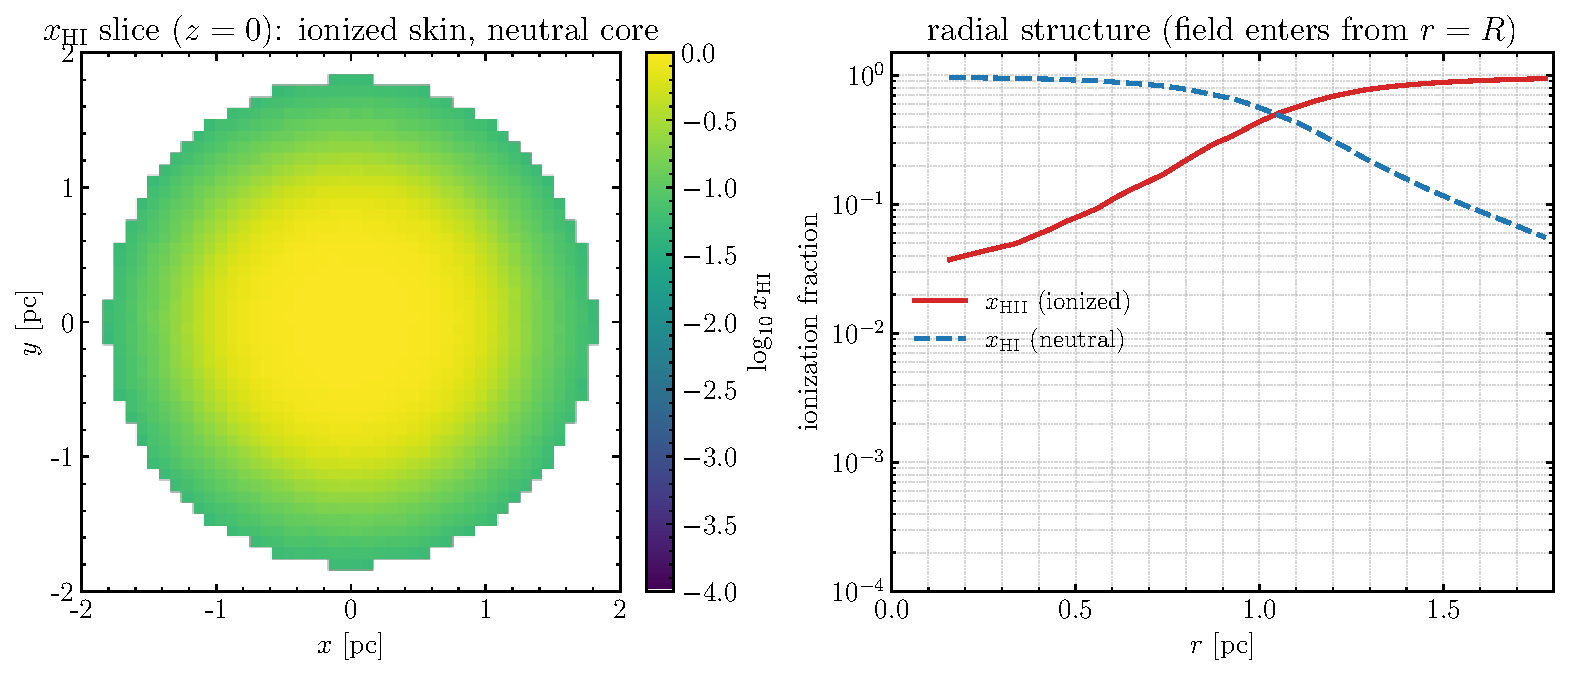
\includegraphics[width=0.95\textwidth]{figures/external_field.pdf}
% source: paper/python/make_external.py, from examples/external_field
\caption{A uniform cloud ($\nH = 1.7\,\mathrm{cm^{-3}}$, $R = 1.8$~pc)
photoionized by an isotropic external radiation field entering the box faces
(a $4\times10^4$~K blackbody shape), with no internal source.  Left: a
planar slice of the neutral fraction $\xHI$ through the cloud center,
showing an ionized skin over a neutral core.  Right: the shell-averaged
radial profiles of $\xHI$ and $x_{\mathrm{HII}}$, with the field entering
at the surface $r = R$.  The ionization structure is the inverse of that
produced by a central source.}
\label{fig:external}
\end{figure*}

\subsection{Opacity and the zero-variance edge walk}
\label{sec:edge}

Each leaf carries the band absorption coefficient
\begin{multline}
  \kappa_b = \nH\big[\xHI\,\sigma_{\mathrm{HI}}(E_b) \\
   + y_{\mathrm{He}}\big(x_{\mathrm{HeI}}\sigma_{\mathrm{HeI}} +
     x_{\mathrm{HeII}}\sigma_{\mathrm{HeII}}\big)(E_b)\big] d_{\mathrm{cm}}
   \;(+\,\kappa_{\mathrm{dust}}),
\end{multline}%
stored as the full $(n_\nu, n_{\mathrm{leaf}})$ array, plus optional metal
photoionization opacity.  Because the ionizing band has no scattering
(without dust) and the diffuse field, when used, is emitted explicitly,
each packet's contribution to the mean-intensity tally is computed
\emph{analytically} along its ray --- the forced-first-flight estimator
of \citet{lucy1999}, made exact:
\begin{equation}
  \Delta J_b(\mathrm{leaf}) = w\,L_{\mathrm{pkt}}\,
  \frac{e^{-\tau_{\mathrm{in}}} - e^{-\tau_{\mathrm{out}}}}{\kappa_b},
  \label{eq:edgewalk}
\end{equation}%
accumulated leaf by leaf until the domain edge.  No interaction sampling
is needed; the only Monte Carlo variance is in the direction and bin
sampling.  From the reduced tally $J_b$ the code forms, for each absorber
$i$, the photoionization rate and photoheating rate
\begin{align}
  \Gamma_i &= \sum_b \frac{[4\pi J\,\Delta\nu]_b\,\sigma_i(E_b)}{h\nu_b},
  \nonumber\\
  \mathcal{H}_i &= \sum_b [4\pi J\,\Delta\nu]_b\,\sigma_i(E_b)
  \left(1 - \frac{E_{\mathrm{th},i}}{E_b}\right).
  \label{eq:rates}
\end{align}

\subsection{Grids: octree AMR and the Cartesian DDA backend}
\label{sec:grids}

\MoCHII{} inherits the \MoCafe{} octree.  The grid may be read as an AMR
leaf list, built from a namelist size ($n_x\times n_y\times n_z$) with an
optional uniform-density sphere or shell, or read from a 3D density cube.
Geometry is fully analytic behind accessor functions, so a leaf's center
and half-size are array reads for a general octree and raster-index decodes
for a uniform Cartesian (``car'') grid --- the same floating-point
expressions in both cases.  The car backend allocates no tree or neighbor
arrays at all (a saving that scales to $\sim$10~GB at $512^3$) and
traverses rays with a dedicated incremental Amanatides--Woo DDA walk, which
is the default for uniform grids.  A verification mode reproduces the
single-level octree traversal bit-for-bit, and the DDA agrees with it to
rounding, at up to twice the transport throughput.  The two backends share
all of the physics, transport, and peel-off code.

\subsection{Ionization and thermal equilibrium}
\label{sec:equil}

In each leaf, the ionization state is solved (\code{solve\_ion\_cell}) from the
ionization rates $R_i = \Gamma_i + \nelec C_i(T)$ and the case-A/B
recombination rates $\alpha_i$: $\xHI = \alpha\nelec/(R_{\mathrm{HI}} +
\alpha\nelec)$, the He chain $n_{i+1}/n_i = R_i/(\alpha_{i+1}\nelec)$, closed
by $\nelec = \nH[x_{\mathrm{HII}} + y_{\mathrm{He}}(x_{\mathrm{HeII}} +
2x_{\mathrm{HeIII}})]$ and solved by a damped fixed point on $\nelec$.  When
thermal balance is enabled, the temperature is updated once each iteration
by finding the root of the net rate $\mathcal{N}(T) = \mathcal{H}(T) -
\mathcal{C}(T)$ by bisection on $\log \Te$; the ionization state is
re-solved at every trial $T$.  The cooling $\mathcal{C}(T)$ assembles
recombination cooling, free-free (with the net ion charge $Z$, including
the trace metals at $Z_{\mathrm{ion}} = \mathrm{stage}-1$), collisional
ionization, \HI{} line cooling, and the trace-metal cooling sum
$\sum \nelec n_{\mathrm{ion}}\Lambda_{\mathrm{ion}}(T)$.  Optional secondary
ionization by fast photoelectrons \citep{shull1985} redistributes the
photoelectron energy between heating and secondary \HI/\HeI{} ionization
in partially neutral gas.

\subsection{The iteration loop and convergence}
\label{sec:iterate}

Each iteration zeroes the band tally, transports the stellar packets
(and, if enabled, rebuilds and transports the diffuse packets), reduces
the tally over MPI, forms the rate integrals, solves each leaf, and
refills the opacity from the new state; the stellar tally is recomputed
from zero each iteration.  Every rank runs the identical cell solves from
the reduced tallies, so all ranks agree on convergence, and only the
node master writes the shared state.

Convergence is measured two ways every iteration, and
\code{par\%conv\_crit} selects which pair controls the loop: the largest
change found in any single cell ($\max|\Delta x_{\mathrm{HII}}|$,
$\max|\Delta \Te|/\Te$) and the volume-integrated measures
\begin{equation}
  \frac{\sum_{\mathrm{leaf}} V\,|\Delta x_{\mathrm{HII}}|}
       {\sum_{\mathrm{leaf}} V\,x_{\mathrm{HII}}},
  \qquad
  \frac{\sum_{\mathrm{leaf}} V\,\nelec\,|\Delta \Te|}
       {\sum_{\mathrm{leaf}} V\,\nelec\,\Te}.
\end{equation}
The volume measures fix two stall modes of these single-cell maxima:
ionization-front jitter occupies little volume (the front shell is a few
thousand cells against $\sim$$10^5$ ionized ones, so its Monte Carlo
noise enters the $L_1$ norm suppressed by that ratio), and the $\nelec$
weight removes the vacuum and no-heating cells whose floor-pinned
oscillation dominates $\max|\Delta \Te|$ in FUV/PDR configurations.  On a
FUV dusty Str\"omgren case at $8\times10^6$ packets, where these single-cell
maxima stall at 0.1 and 6.4, the volume measures decay smoothly
to Monte Carlo floors of $2.7\times10^{-3}$ and $6.6\times10^{-3}$ by
iteration $\sim$27, and 30 further iterations leave the ionized volume
unchanged to 0.014\%.  The floors scale as $1/\sqrt{N_{\mathrm{packets}}}$,
and the volume criterion is the recommended production setting.

\subsection{Explicit diffuse field}
\label{sec:diffuse}

When the explicit diffuse field is enabled, case-B OTS is replaced by
case-A rates plus explicit emission of ground-recombination packets in
three channels (\HII, \HeII, \HeIII) with rate $\alpha_1 = \alpha_A -
\alpha_B$.  Detailed balance fixes the emitted spectrum: per unit photon
energy the free--bound photon emissivity of each ground continuum is
\begin{equation}
  n(E) \;\propto\; E^{2}\,\sigma_{\mathrm{pi}}(E)\,
     \exp\!\left[-\frac{E - E_{\mathrm{th}}}{kT_e}\right],
  \qquad E \ge E_{\mathrm{th}},
  \label{eq:milne}
\end{equation}
evaluated with the \emph{same} ground-state photoionization cross section
the transport absorbs with, so a packet is absorbed with the cross section
it was emitted with.  Restoring the Milne prefactor turns the integral of
Equation~(\ref{eq:milne}) into $\alpha_1(T)$ itself, which recovers
$\alpha_{1s}(\HI, 10^4~\mathrm{K}) = 1.579 \times 10^{-13}$~cm$^3$\,s$^{-1}$
against the tabulated $1.58 \times 10^{-13}$.  \MoCHII{} takes $\alpha_1$
from that integral, so the case A/B split, the emitted spectrum and the
packet count all rest on one cross section; the code reports the integral
against the $\alpha_A - \alpha_B$ used for the emission rate without
rescaling either, and the two agree to $0.01$\% on all three channels.
Because packets
are equal-energy and their number follows the channel's \emph{energy}
luminosity, their energies are drawn from $E\,n(E)$ rather than $n(E)$,
which makes the represented photon rate exactly $n_e n_{\rm ion}\alpha_1 V$.
The cumulative distribution is tabulated in $x = (E-E_{\mathrm{th}})/kT$,
interpolated in $\log T$ and inverted once.  A near-threshold approximation
$E = E_{\mathrm{th}} + kT_e\,x$ with $x \sim \mathrm{Exp}(1)$, which is
Equation~(\ref{eq:milne}) with the $E^2\sigma_{\rm pi}$ weight dropped, is
retained as an option.  The emission table is rebuilt from the current state
each iteration; packets are transported by the same edge walk.  The
sampled photon energy is mapped to its bin by a binary search of the
stored bin-edge array, correct on both the aligned and the plain
logarithmic grids: an
energy exactly on a threshold edge falls in the bin \emph{above} it, the
physically correct side for a recombination photon emitted just above
threshold.

An optional fourth channel adds the \HeI{} excited-level recombination
radiation.  Every case-B \HeII{} recombination reaches $1^1$S through
exactly one of the $n=2$ terms, so what the channel needs are the three
branch fractions; their absolute scale is already set by $\alpha_B(\HeII)$.
They are formed from one internally consistent set of effective
recombination coefficients,
$2.10\times10^{-13}\,T_4^{-0.381}$ ($2^3$S),
$2.06\times10^{-14}\,T_4^{-0.451}$ ($2^1$S) and
$4.17\times10^{-14}\,T_4^{-0.695}$ ($2^1$P) $\cmc$, from
\citet[][Table~1, with J.~S.~Mathis]{benjamin1999} as tabulated in K.~Wood's
\code{ionize} \citep{wood2004} and in \textsc{CMacIonize}
\citep{cmacionize2018}, normalized by their sum.  Taking all three from one
source matters more than the individual values, because a ratio of
coefficients with unrelated temperature dependences is not a branch fraction;
normalizing by the sum rather than closing one branch against an external
$\alpha_B$ keeps the mismatch between two independent data sets out of
whichever branch is solved last.  That sum is $0.90\,\alpha_B(\HeII)$ at
8000~K and $0.97$ at $10^4$~K, and the shortfall is reported at start-up
rather than absorbed.  At 8000~K the fractions are $0.762 : 0.076 : 0.162$
against the $0.750 : 0.083 : 0.167$ of the low-density statistical weights
($0.741 : 0.076 : 0.183$ at 5000~K, $0.771 : 0.076 : 0.153$ at $10^4$~K): a
modest temperature-dependent correction, not a reordering.  The $2^1$S
photons are drawn from the tabulated \citet{drake1969} two-photon
distribution rather than flat above the \HI{} edge; that shape also fixes the
H-ionizing fraction, 0.5564 photons per decay with a mean in-band energy of
16.11~eV.  Together the two replace the 19.200~eV in 0.9634 photons that the
statistical weights and a flat two-photon spectrum emit per case-B \HeII{}
recombination by 19.223~eV in 0.9663 photons at 8000~K.  The 584~\AA{}
photon of the $2^1$P branch is a resonance photon, and two irreversible
outcomes compete during its trapped random walk: absorption by a hydrogen
atom, which photoionizes it, or collisional conversion
$2^1$P\,$\to$\,$2^1$S in the helium atom that last absorbed it, after which
the decay leaves as the two-photon continuum instead.  \MoCHII{} splits the
branch with the escape probability that \citet{wood2004} and
\textsc{CMacIonize} \citep{cmacionize2018} adopt,
$p_{584} = [1 + 77\,x(\mathrm{He^{0}})/(\Te^{1/2}\,x(\mathrm{H^{0}}))]^{-1}$
with $\Te$ in K; it is a property of the emitting leaf, so it folds into the
branch weights of the emission table and costs no further random variate.  A
converted decay radiates 20.62~eV as the two-photon pair, the remaining
0.60~eV leaving as the non-ionizing 2.06~$\mu$m $2^1$P\,$\to$\,$2^1$S line.
The same probability sets the effective coefficient of the \HeI{} two-photon
nebular continuum,
$\alpha_{2q} = \alpha(2^1\mathrm{S}) + (1-p_{584})\,\alpha(2^1\mathrm{P})$,
so the transported packets and the tabulated continuum describe one nebula.
Emission-weighted $p_{584}$ is $0.12$ at HII40 and $0.004$ at HII20: most of
the branch converts, the channel loses 7--8\% of its photons and softens,
and the fronts move inward --- at HII40 by $-0.0036$~pc in \HeI{} and
$-0.0100$~pc in \HI{}, with $L(\mathrm{H}\beta)$ down $0.20\%$.  At HII20
the softer spectrum leaves little \HeII{} to recombine, so the channel
carries $2\%$ of the diffuse field rather than $18\%$ and the same fronts
move by $-0.0002$~pc.

Four corrections to what the diffuse field emits have now been made --- the
Milne ground-continuum shape, the \citet{drake1969} two-photon spectrum, the
effective branch coefficients and the 584~\AA{} fate --- and at HII40 they
displace the \HeI{} front by $+0.0006$, $-0.0003$, $+0.0002$ and
$-0.0036$~pc, a net $-0.0031$~pc.  Each is separately required, and each
reproduces an external implementation or an exact relation; together they
recover under $2\%$ of the $0.18$~pc by which that front sits inside the
\textsc{Cloudy} c25.00 one, and they move it the wrong way.  The remaining
code-to-code difference of Section~\ref{sec:hii} is therefore not in what
the diffuse field emits.  Neither of the two axes those corrections left open
can reach it either.  Diffuse transport is bounded by its own extremes:
explicit transport puts the front at 4.1197~pc and the on-the-spot
approximation at 4.1816~pc, a total range of 0.062~pc, with \textsc{Cloudy}
0.124~pc beyond the nearer end.  The \HeI{} ground-continuum atomic data are
bounded by measured sensitivity: scaling $\sigma_{\rm pi}$(\HeI) or the \HeI{}
recombination rate by $3\%$ moves the front by $0.008$ and $0.024$~pc, so
$0.18$~pc would take $70\%$ and $23\%$.  Outside the diffuse field, the
source photon budget reproduces the \textsc{Cloudy}
$Q({>}13.6~\mathrm{eV})$ and $Q({>}24.6~\mathrm{eV})$ to $0.003\%$, and the
benchmark runs dust free.
What the residual does have is a signature: $x(\mathrm{H^{0}})$ agrees with
\textsc{Cloudy} to 1--2\% throughout the ionized zone, while the
$x(\mathrm{He^{0}})$ ratio grows monotonically outward, 1.007 at 1.6~pc to
1.196 at 3.8~pc.  That is not a normalization offset, which would be
radius-independent, but a small helium-specific difference compounding with
depth, as it must when He$^{0}$ carries 84--96\% of the opacity above
24.6~eV and $24\%$ of the He-ionizing supply is taken by other absorbers.
Closing $4.1\%$ in radius is $13\%$ in volume, asking for $14\%$
in $Q(\mathrm{He^{0}})$ or $20\%$ in $\alpha_B$(\HeI), and neither is
available.

That bounding exercise did expose one defect.  $\alpha_1$ had been taken
from a level-resolved fit \citep{mao2016} while $\alpha_A$ came from the
Badnell total, so $\alpha_B = \alpha_A - \alpha_1$ crossed two unrelated
determinations; \textsc{Cloudy} c25.00 \citep{cloudy2025}, which derives the
same quantity level by level from its own cross sections through the Milne
relation, puts that fit $2.4\%$ low for \HeI.  Replacing it by the Milne
integral over the transport cross sections brings all three channels within
$0.35\%$ of \textsc{Cloudy} and the start-up cross-check from $3.4\%$ to
$0.01\%$.  The front moves outward by $0.008$~pc, leaving the residual at
$0.178$~pc; $L(\mathrm{H}\beta)$ falls $0.4\%$, marginally further from the
published values, which is recorded but is not an argument against restoring
an exact relation.

The helium ionization network has since been compared network to network,
and it does not supply the residual either.  At $10^{4}$~K,
$\alpha_A$(\HeI) is $4.358 \times 10^{-13}\,\cmc$ in \textsc{Cloudy}'s
explicit sum over levels, $4.372$ in \MoCHII, $4.263$ in the effective
coefficients of \citet{benjamin1999} used by \citet{wood2004} and
\textsc{CMacIonize}, and $4.839$ in \textsc{Mocassin}'s Verner \& Ferland
(1996) fit.  No code truncates the cascade --- all three treatments run over every
level --- and the $11\%$ spread is confined to \HeI: the one-electron species
agree to $0.7\%$ (\HI) and $0.3\%$ (\HeII), where an exact analytic solution
leaves nothing to disagree about, so what spreads is the two-electron atomic
data itself.  \MoCHII{} sits within $0.3\%$ of \textsc{Cloudy}, which also
means any helium comparison against \textsc{Mocassin} inherits that
difference.  The \HeI{} excited levels a resolved model atom carries lie
below \MoCHII's 13.598~eV band floor and are worth $0.2$--$0.6\%$ of extra
ionization.  Nor is the metal opacity, the one candidate outside helium,
large enough: scaling the summed metal cross section by $\pm30\%$ moves the
front $+0.031$ and $-0.072$~pc, an asymmetric and saturating response worth
$0.103$~pc per unit fractional increase, so $0.178$~pc would need $+180\%$
against cross sections that reproduce the \citet{verner1996} fits to
$10^{-6}$.

The residual is therefore unexplained while every single-parameter
explanation for it is quantitatively excluded.  What is untested is a
combination of several few-percent differences --- in the \HeI{}
recombination rate, in the shape of $\sigma_{\rm pi}$(\HeI), in the metal
opacity of the 21--40~eV window --- acting together through the He$^{0}$
optical depth, which compounds them with depth exactly as the signature
shows, and which no experiment varying one ingredient at a time can
reproduce.  At HII40 the diffuse band luminosity
converges to $\sim$$0.5\,L_\star$.

\subsection{Quasi-random photon launching}
\label{sec:qmc}

Optionally the packet launch draws its variables (source component, photon
energy through the source CDF in continuous mode or frequency bin in grouped
mode, direction, and any entry-surface coordinates) from an
Owen-scrambled Sobol sequence \citep{joekuo2008,burley2020} instead of the
Mersenne Twister, while every post-launch transport event stays
pseudo-random.  The Sobol point is addressed by the \emph{global} photon
number, so the launch set is independent of the MPI task count.  Because
the ionizing band has no scattering, the direct field is an analytic
function of the launch variables (Eq.~\ref{eq:edgewalk}), and a
low-discrepancy launch set reduces its noise directly.

Figure~\ref{fig:qmc} shows the resulting scaling on the fixed-state
analytic-attenuation test.  The Monte Carlo cell-wise root-mean-square error
in $\Gamma_{\mathrm{HI}}$ follows the $N^{-1/2}$ reference slope while the
Owen-scrambled Sobol launch follows $N^{-1}$, so the effective photon gain,
the ratio of the two variances, grows with the packet count: $28.8\times$ at
$N = 2^{17}$, $66.7\times$ at $2^{18}$, $143\times$ at $2^{19}$, and
$231\times$ at $2^{20}$.  The two launch sets cost the same wall time, and
the quasi-random result carries no significant bias: its mean $|$bias$|$ is
$0.011$--$0.012\%$, and the $0.06\%$ that an earlier reference showed was that
reference carrying a fitted H\,\textsc{i} cross section where the run uses the
exact hydrogenic one.

\begin{figure}[t]
\centering
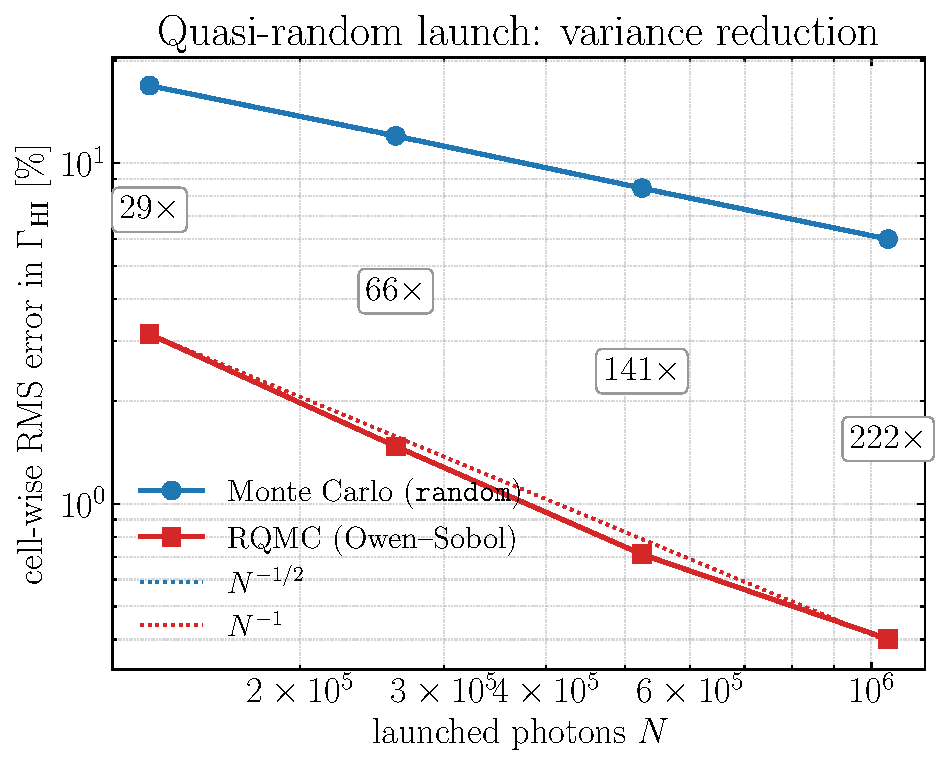
\includegraphics[width=\columnwidth]{figures/qmc_variance.pdf}
% source: paper/python/make_qmc.py, from tests/qmc/v3/
\caption{Quasi-random photon launching.  Cell-wise root-mean-square error
in $\Gamma_{\mathrm{HI}}$ on the fixed-state analytic-attenuation test, as a
function of the launched photon count $N$, for the ordinary Monte Carlo
(\texttt{random}) and Owen-scrambled Sobol (RQMC) launches, with the
$N^{-1/2}$ and $N^{-1}$ reference slopes.  The boxed labels give the
effective-photon gain (the variance ratio) at each $N$, which grows with $N$
as the two slopes diverge.}
\label{fig:qmc}
\end{figure}

\subsection{Peel-off imaging}
\label{sec:peel}

After convergence, one extra transport pass runs with observer peeling
(the \MoCafe{} convention adapted to the band).  Every emitted packet
peels a direct contribution $L_{\mathrm{pkt}}\,w\,e^{-\tau}/(4\pi r^2)$
toward each observer, and, when dust scattering is sampled, every
interaction peels a scattered contribution with the Henyey--Greenstein
phase function.  The optical depth to the box edge is integrated by a
tally-free walk, so the images carry exactly the transport's extinction.
Images are TAN projections written as surface brightness, split into
direct/scattered and ionizing/FUV channels; with a spectral cube option
the channel axis becomes the band bin for hardness maps.  Leaf-resolved
line and continuum emissivities are also written, from which
flux-conserving line and field maps are produced.

Figure~\ref{fig:peel} is an example: the FUV channel of a dusty,
radiation-bounded \HII{} region with a central star, seen by the observer.
The direct image is the attenuated stellar point source (peak
$\log_{10} I = 1.95$ in $\mathrm{erg\,s^{-1}\,cm^{-2}\,sr^{-1}}$), and the
scattered image is the dust halo it illuminates (peak $0.24$, covering some
$27\%$ of the pixels).  The halo is the observer-dependent component that a
one-dimensional or angle-averaged calculation does not provide, and the sum
of the two is the surface brightness an observer measures.  The ionizing band contributes almost nothing to the
scattered image here, because in a bounded nebula it is absorbed before it
can scatter out.  Alongside the extincted image the code also writes the
bin-resolved image cube and an unattenuated (\code{direc0}) image, the
latter giving a line-of-sight optical-depth map as its ratio to the
extincted one.

\begin{figure*}[t]
\centering
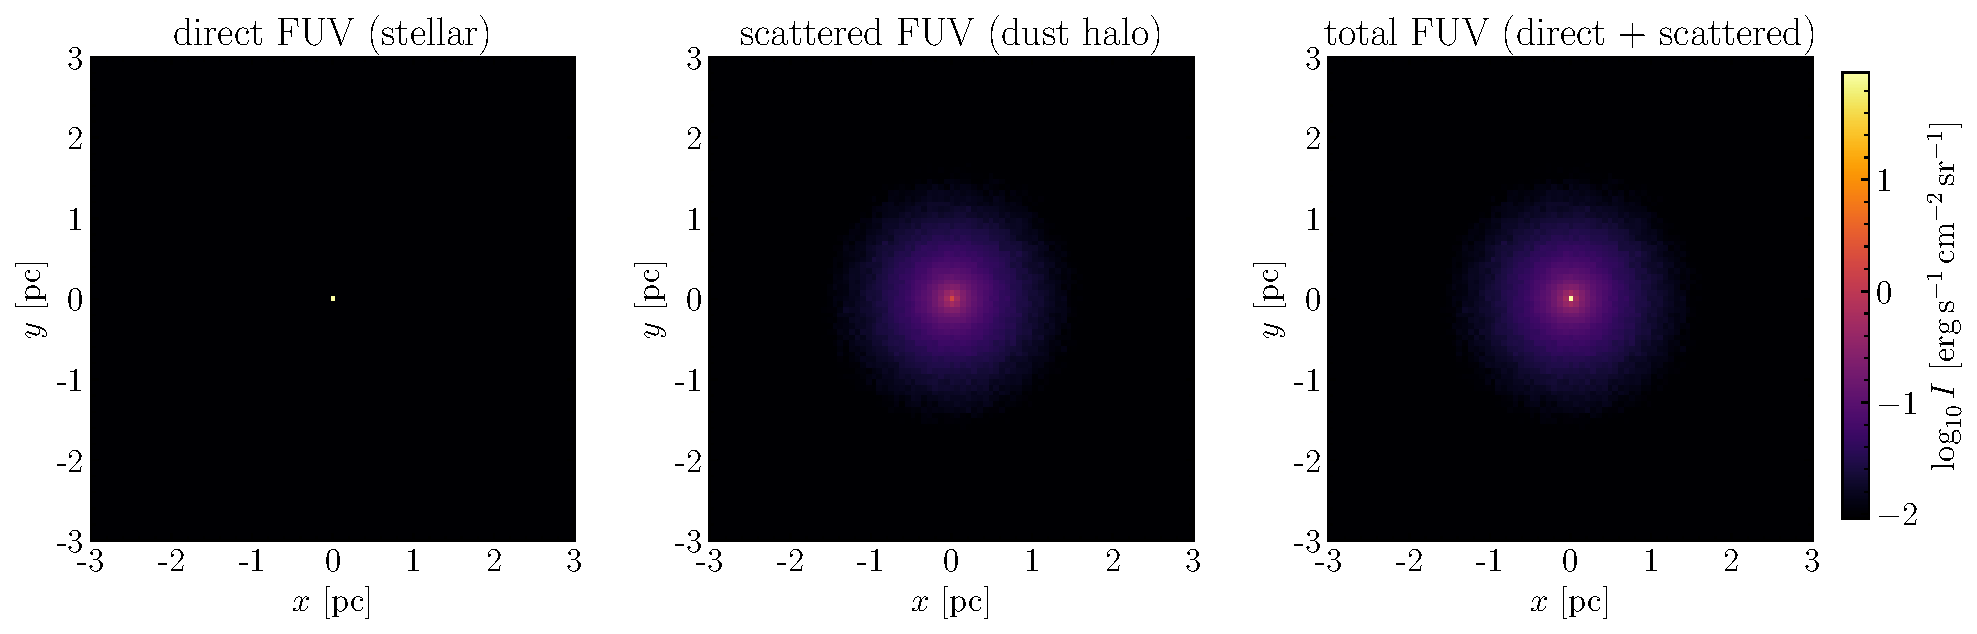
\includegraphics[width=\textwidth]{figures/peel.pdf}
% source: paper/python/make_peel.py, from tests/peel/peel_scat
\caption{Peel-off synthetic imaging of a dusty, FUV-illuminated \HII{}
region with a central star, in the FUV channel.  Left: the direct stellar
image, an attenuated point source.  Center: the dust-scattered halo, the
observer-oriented contribution.  Right: their sum, the synthetic
observation.  All three panels share one logarithmic scale of the specific
intensity $I$ integrated over the channel's band, so the extended scattered
halo is directly comparable to the compact direct source.}
\label{fig:peel}
\end{figure*}

%==========================================================================
\section{Atomic data}
\label{sec:atomic}

The design principle for the atomic data is that adding an ion is a
\emph{data operation, not a code operation}.  All rate coefficients are
fitted offline by a Python pipeline from CHIANTI v11.0.2
\citep{dere1997,delzanna_chianti} and the Strathclyde/Badnell tables, and
are evaluated online by fixed analytic formulae.  Every coefficient file
carries a provenance header (source, version, fit range, maximum fit
error), so the coefficients are auditable and the Fortran only evaluates
formulae.

\subsection{Photoionization cross sections}
\label{sec:xsec}

The one-electron ions \HI{} ($Z=1$) and \HeII{} ($Z=2$) use the exact
ground-state hydrogenic cross section \citep{osterbrock2006}
\begin{gather}
  \varepsilon = \sqrt{E/E_{\mathrm{th}}-1},
  \nonumber\\
  \sigma(E) = \frac{\sigma_0}{Z^2}\left(\frac{E_{\mathrm{th}}}{E}\right)^{4}
  \frac{\exp\!\big(4 - 4\arctan\varepsilon/\varepsilon\big)}
       {1 - e^{-2\pi/\varepsilon}},
  \label{eq:sighyd}
\end{gather}%
with $\sigma_0 = 6.30\times10^{-18}\,\mathrm{cm^2}$ and $E_{\mathrm{th}}$
the true ionization potential (13.598 and 54.416~eV), tied to the physical
edge so it stays aligned with the band grid.  \HeI{} and every metal ion
use the single-shell analytic fit of \citet{verner1996}:
\begin{gather}
  x = \frac{E}{E_0} - y_0,\qquad z = \sqrt{x^2 + y_1^2},
  \nonumber\\
  \sigma(E) = \sigma_0\left[(x-1)^2 + y_w^2\right]
  z^{-Q}\left(1 + \sqrt{z/y_a}\right)^{-P},
  \nonumber\\
  Q = 5.5 - \tfrac{1}{2}P,
  \label{eq:vfky}
\end{gather}%
with parameters parsed directly from the authors' \code{phfit2.f} table.
For the elements absent from that table (P, Cl, K --- Opacity-Project
gaps), the \citet{verner1995} outer-shell subshell fit is used instead,
the same hybrid as \textsc{Mocassin}.  The cross sections are cross-checked
against the independent implementation in the exoplanet-atmosphere code
EXHALE.

\subsection{Recombination}
\label{sec:recomb}

The default recombination model takes the total (case-A) radiative
recombination $\alpha_A$ from the \citet{badnell2006} radiative
recombination fit,
\begin{gather}
  \alpha_{\mathrm{RR}}(T) =
  \frac{A}{\sqrt{T/T_0}\big(1+\sqrt{T/T_0}\big)^{1-b}
           \big(1+\sqrt{T/T_1}\big)^{1+b}},
  \nonumber\\
  b = B + C\,e^{-T_2/T},
  \label{eq:badnellrr}
\end{gather}%
the ground-level ($n=1$) direct-capture rate $\alpha_1$ from the Milne
relation applied to the same photoionization cross sections the transport
absorbs with (Section~\ref{sec:diffuse}), and forms case B by
removing the ground term, $\alpha_B = \alpha_A - \alpha_1$.  It is
evaluated at run time from the seven-coefficient form of \citet{mao2016}
with coefficients refitted to that integral; the $\HeII\to\HeI$ channel
adds the Badnell three-term dielectronic sum.  This
construction mirrors how \textsc{Cloudy} splits case A and case B (total
minus resolved ground) and reuses the same modern data.  An alternative
setting selects the \citet{huignedin1997} fits; the two agree to $<$0.6\% for
\HII{} and \HeIII{}, the one substantive difference being
$\HeII\to\HeI$, where the Badnell value ($4.37\times10^{-13}\,\cmc$ at
$10^4$~K) is $\sim$5\% higher in case B and coincides with
\textsc{Cloudy}, while the older \citet{huignedin1997} value is low and the
\textsc{Mocassin} Verner \& Ferland value ($4.84$) is the high outlier.
For the metal cascade, total recombination is the \citet{badnell2006}
radiative recombination plus the Badnell-group dielectronic fits
$\alpha_{\mathrm{DR}}(T) = T^{-3/2}\sum_i c_i e^{-E_i/T}$
\citep{badnell2003}, read from the Strathclyde tables (verified md5-identical
to the copies \textsc{Cloudy} redistributes), with a CHIANTI fallback for
the few ions Badnell does not tabulate.

\subsection{Collisional ionization and charge exchange}
\label{sec:ci}

Collisional ionization uses the \citet{voronov1997} fit
\begin{equation}
  k(T) = A\,\frac{1 + P\sqrt{U}}{X + U}\,U^{K} e^{-U},
  \qquad U = \frac{\Delta E}{kT},
\end{equation}%
with an optional hybrid that multiplies each rate by the constant
\citet{dere2007}/Voronov ratio of that element and stage; the difference matters
only in shielded, low-ionization zones where collisions are the sole
metal-ionization channel.  Charge exchange with hydrogen uses
\citet{huang2023} Table~4 for the first stages and the
\citet{kingdon1996} fits $k = a\,T_4^{b}(1 + c\,e^{d\,T_4})$ for the higher
stages (recombination direction).  The tabulated higher-stage rates are
indexed by the \emph{product} ion of the reaction
$\mathrm{X}^{i+} + \mathrm{H}^{0} \to \mathrm{X}^{(i-1)+}$, a convention worth
stating explicitly because it is easy to misread by one ionization stage and
because the doubly and triply ionized metal fractions are sensitive to it;
the indexing used here is checked against \textsc{Mocassin}'s ionization loop
and \textsc{CMacIonize}.

\subsection{Cooling and $n$-level diagnostic data}
\label{sec:cooldata}

Collisional line cooling enters the code at two levels, both built from the
same CHIANTI v11.0.2 model of each ion (level energies from the observed
term structure, radiative $A$-values, and effective collision strengths
descaled after \citealt{burgess1992}).  The thermal loop needs a cooling
rate at every trial temperature of the bisection, and therefore uses a
closed-form fit suppressed to the local density (below); the diagnostic
output needs density-dependent emissivities, and therefore solves the level
populations.  Both are the same statistical-equilibrium solution of each
ion, so the thermal balance and the emergent line list are one physics.

The thermal-loop coefficient is a multi-exponential fit
\begin{equation}
  \Lambda_{\mathrm{ion}}(T) = T^{-1/2}\sum_{i=1}^{N} A_i\,e^{-T_i/T}
  \quad [\mathrm{erg\,cm^3\,s^{-1}}],
  \label{eq:cool}
\end{equation}%
a rate coefficient multiplying $\nelec n_{\mathrm{ion}}$, fitted over
$10^3$--$10^5$~K to the $\nelec \to 0$ limit of that ion's own
statistical-equilibrium solution --- all population in the lowest level,
excitation at the observed level energies, and the full cascade energy
radiated.  The maximum fit error over the temperatures that carry the
cooling is $2.2\%$ across the default C/N/O/Ne/S set (the coefficients of
every ion are distributed with the code, Appendix~\ref{app:atomic}; the
heavily depleted Si/Cl/Ca ions have larger full-range fit errors, confined
to the temperature tails where the cooling contribution is negligible).

By itself Eq.~(\ref{eq:cool}) carries no collisional de-excitation, so it is
exact for lines whose critical density is far above the local $\nelec$ and
increasingly too large for those below it --- the far-infrared
fine-structure transitions [O\,\textsc{iii}] 52 and 88\,$\mu$m and
[C\,\textsc{ii}] 158\,$\mu$m, whose electron critical densities are
$10^{2}$--$10^{3.5}\,\mathrm{cm^{-3}}$, so at the
$\nelec \sim 10^2\,\mathrm{cm^{-3}}$ of an \HII{} region it overestimates
the line-cooling budget by about $12\%$ (Section~\ref{sec:coolcheck}).  The
thermal loop therefore suppresses the coefficient to the local density.  A
$(\Te, \nelec)$ table, built once at setup by solving the same $n$-level
atom over a grid and stored as the ratio
$\Lambda_{\mathrm{SE}}(\Te,\nelec)/\Lambda_{\mathrm{SE}}(\Te,\nelec\!\to\!0)$,
multiplies Eq.~(\ref{eq:cool}) at each trial temperature; the fraction of the
low-density cooling the (often truncated) $n$-level model does not resolve
--- its high-excitation resonance lines, of far higher critical density ---
is left unsuppressed, and as $\nelec\to0$ the suppression is unity and the
coefficient returns to the fit exactly.  Every ion carrying a cooling fit
also carries an $n$-level model, so none is left in the zero-density limit;
the two neutrals C\,\textsc{i} and N\,\textsc{i} are the most strongly
suppressed of all, their far-infrared fine-structure lines having
$n_{\rm crit}$ of only a few $\mathrm{cm^{-3}}$.  This density-suppressed cooling
(\code{cooling\_model = local\_ne}, the default) is built from the very
solve that produces the diagnostic lines, so the two are one physics; the
pure zero-density fit is retained as the \code{low\_density} option, exact
in the diffuse gas the limit is written for, and the planetary-nebula
densities of Section~\ref{sec:summary} require the table in any case.

For the
output-time diagnostics, the lowest $n$ levels, radiative $A$-values, and
effective collision strengths $\Upsilon(T)$ (low-order Chebyshev fits in
Burgess--Tully scaled space; worst transition 1.7\%,
Table~\ref{tab:tier2}) are exported for the line-emitting ions of the
eleven-element registry.  A statistical-equilibrium solve at output time
(\code{nlevel\_mod}) uses these to compute the collisional emission-line
luminosities exactly --- the density-dependent emissivities the
low-density cooling fits cannot provide.  The fitted files reproduce direct
CHIANTI spline evaluations of the classic diagnostic ratios to 0.05--0.5\%,
and the Fortran solver matches an independent Python reference solver to
four significant digits.  PyNeb cross-checks give [\textsc{O\,iii}]
5007/4363 to 1.2\% and [\textsc{N\,ii}] 6584/5755 to 0.3\%; the density
diagnostics and the iron lines differ by up to 6--16\% from PyNeb's
independent collision data --- the well-known database spread, a
data-vintage bracket rather than a code error.

\subsection{Recombination lines and the nebular continuum}
\label{sec:reclines}

Hydrogen and \HeII{} recombination-line emissivities are interpolated from
the \citet{storey1995} case-A/B tables (following \code{par\%case\_ab}),
and \HeI{} lines from the \citet{porter2012,porter2013} case-B
collisional-radiative emissivities.  The nebular continuum combines the
free-bound plus free-free coefficients of the MOCASSIN
\citep{ercolano2006} tables with a Milne extension above the edges and the
three two-photon continua; the free-free Gaunt factor is the
\citet{hummer1988} fit, with the \citet{vanhoof2014} table as a drop-in
option (the two agree to a median $5\times10^{-5}$ in $\Te$).

\subsection{The \HeI{} \texorpdfstring{$2^3$S}{2 3S} metastable diagnostic}
\label{sec:heimeta}

The metastable $2^3$S level of neutral helium is the lower level of the
10833~\AA\ triplet, whose absorption traces the extended atmospheres of
close-in exoplanets and the neutral gas of nebulae.  In \HII{} regions the
triplet is seen in emission, and near-infrared spectrographs such as
NIRSPEC, CARMENES, and X-Shooter resolve its profile in Galactic regions
like M17-B and NGC 3603 and in extragalactic star-forming regions
\citep{draine2026}.  \MoCHII{} solves its
population leaf by leaf on the converged state, following the balance of
\citet{oklopcic2018}: recombination into the triplet ladder and collisional
feeding from the ground state populate $2^3$S, while radiative decay,
collisional de-excitation, Penning ionization by neutral hydrogen, and
photoionization by the transported radiation field depopulate it.  From the
resulting density the line-center optical depth of the 10833~\AA\ doublet is
formed.  The diagnostic is pure post-processing, with no feedback on the
ionization or thermal balance.

Figure~\ref{fig:hei10833} shows both sides of the transition for a dense
compact example ($\nH = 10^4\,\mathrm{cm^{-3}}$, $R = 0.15$~pc, $\Te$ fixed
at $10^4$~K).  On the absorption side, the $2^3$S column density reaches
$N = 3.4\times10^{15}\,\mathrm{cm^{-2}}$ and the line-center optical depth of
the blended $J' = 1, 2$ doublet reaches $4.1\times10^{3}$ on the central
sightline, falling through $\tau_0 = 1$ only at a projected radius of
$0.139$~pc, so all but the outermost rim of the projected disk is optically
thick at 10833~\AA.  Such a column makes the line resonantly scatter, as
\citet{draine2026} shows for \HII{} regions: repeated scattering broadens the
emergent profile into a multipeaked feature whose width can exceed
$100\,\mathrm{km\,s^{-1}}$ and whose centroid is blueshifted by up to
$\sim$$14\,\mathrm{km\,s^{-1}}$ relative to other lines, while the extended
path length lets dust absorb a larger share of the photons and so weakens the
line.  The He\,\textsc{i} 10833/Pa$\gamma$ ratio therefore stops being a clean
He$^{+}$/H$^{+}$ measure once the metastable column is large.  The
optically-thin diagnostic likewise underestimates the true absorption over
most of the region, which is what makes the $2^3$S output of
Figure~\ref{fig:hei10833} the input to a scattering calculation rather than an
observable in itself.  That calculation is within reach: the converged $2^3$S
density is handed to \textsc{LaRT}
\citep{seon2020,seon2022,seon2024}, a Monte Carlo resonant-line transfer code
that already carries a 10833~\AA\ module and has been applied to the line in
an exoplanet atmosphere \citep{yan2022}.  The coupling is in place --- a
converter writes the \MoCHII{} metastable grid in \textsc{LaRT}'s input
format, and the two codes agree on the line-center optical depth of the
example above to $0.5\%$ --- and the resonant-scattering profiles will be
presented in a forthcoming paper.  On the
emission side, the same
transition radiates the 10833~\AA\ line, and the code writes its emissivity
from the \citet{porter2012} recombination table --- a collisional-radiative
total, so it is used as tabulated and nothing is added to it.  Integrated, the
line carries $1.34\,L(\mathrm{H}\beta)$ here, and its emissivity falls at
$r \simeq 0.13$~pc, inside the ionized sphere: the He$^{+}$ zone ends where
the $>$24.6-eV photons run out, while hydrogen stays ionized to $0.15$~pc.

\begin{figure*}[t]
\centering
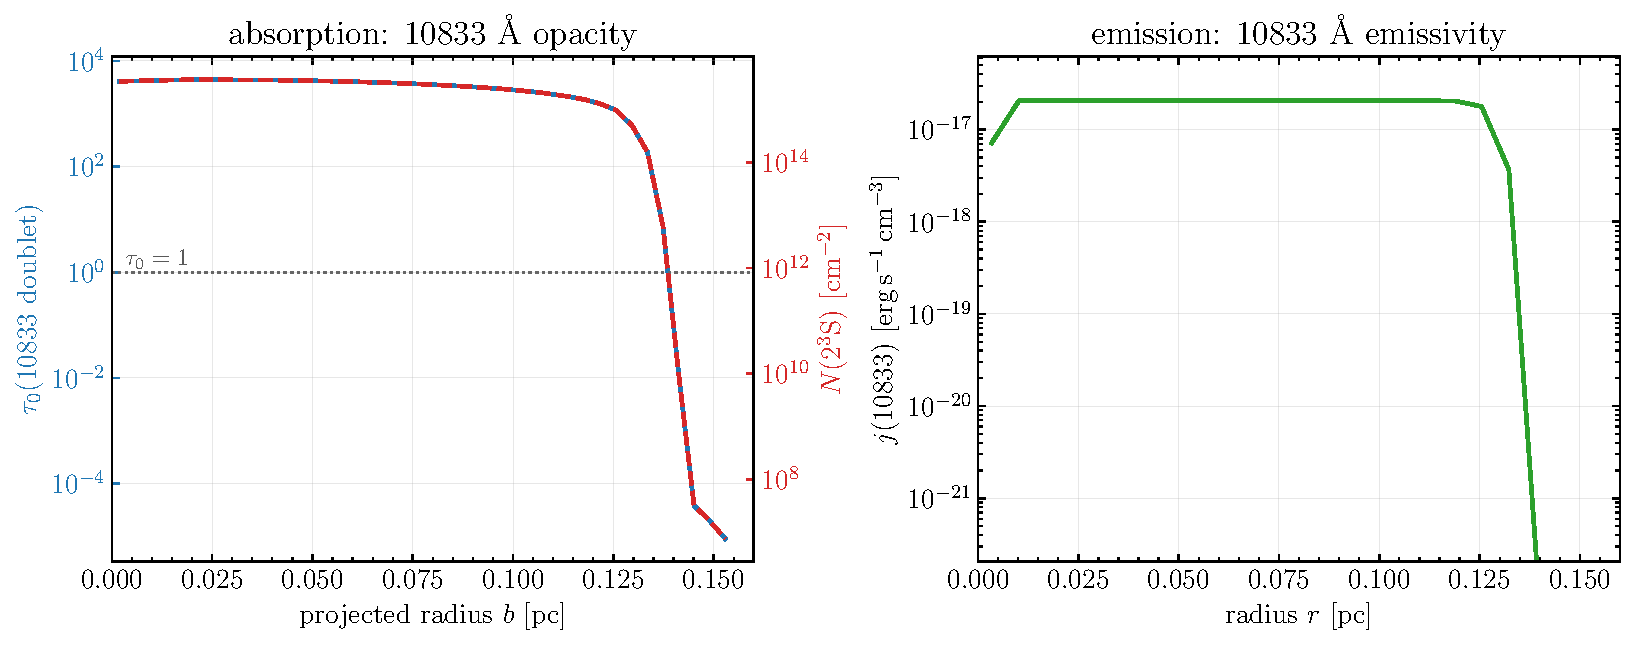
\includegraphics[width=0.95\textwidth]{figures/hei10833.pdf}
% source: paper/python/make_hei10833.py, from examples/hei_metastable/hei_high_density
\caption{The \HeI{} $2^3$S metastable diagnostic for a dense compact
example ($\nH = 10^4\,\mathrm{cm^{-3}}$, $R = 0.15$~pc, $\Te = 10^4$~K), as
radial profiles of the two sides of the same $2^3{\rm S}$--$2^3{\rm P}$
transition.  Left, absorption: the 10833~\AA\ line-center optical depth
$\tau_0$ of the blended $J' = 1, 2$ doublet against projected radius (left
axis) with the $2^3$S column density on the right axis.  Both are
line-of-sight integrals, and at the fixed $\Te$ of this run the Doppler width
is constant, so the two are strictly proportional and the right axis is the
conversion of the left; the curves overlie.  The region is optically thick
inside $b = 0.139$~pc, where the optically-thin diagnostic breaks down.
Right, emission: the 10833~\AA\ emissivity against radius, from the
\citet{porter2012} He\,\textsc{i} block of the emissivity file.}
\label{fig:hei10833}
\end{figure*}

%==========================================================================
\section{Validation}
\label{sec:validation}

\MoCHII{} is validated against analytic solutions, an exact 1D reference
solver, and the Lexington benchmark suite, in staged tests.  Each
AMR result is required to reproduce the equivalent uniform-grid run.

\subsection{Rate integrals and the Str\"omgren sphere}
\label{sec:stromgren}

The zero-variance edge walk (Eq.~\ref{eq:edgewalk}) is verified on a
uniform sphere ($\nH = 1$, $R = 1$~pc, $\xHI = 0.1$) with a central
$10^5$~K source.  Against the cell-volume-averaged analytic attenuation,
$\Gamma_{\mathrm{HI}}$ has a mean bias of $+0.08\%$ and a median deviation
of $0.38\%$ (pure Monte Carlo noise), and $\Gamma_{\mathrm{HeI}}$ a bias of
$+0.011\%$ (Figure~\ref{fig:g0}).

\begin{figure}[t]
\centering
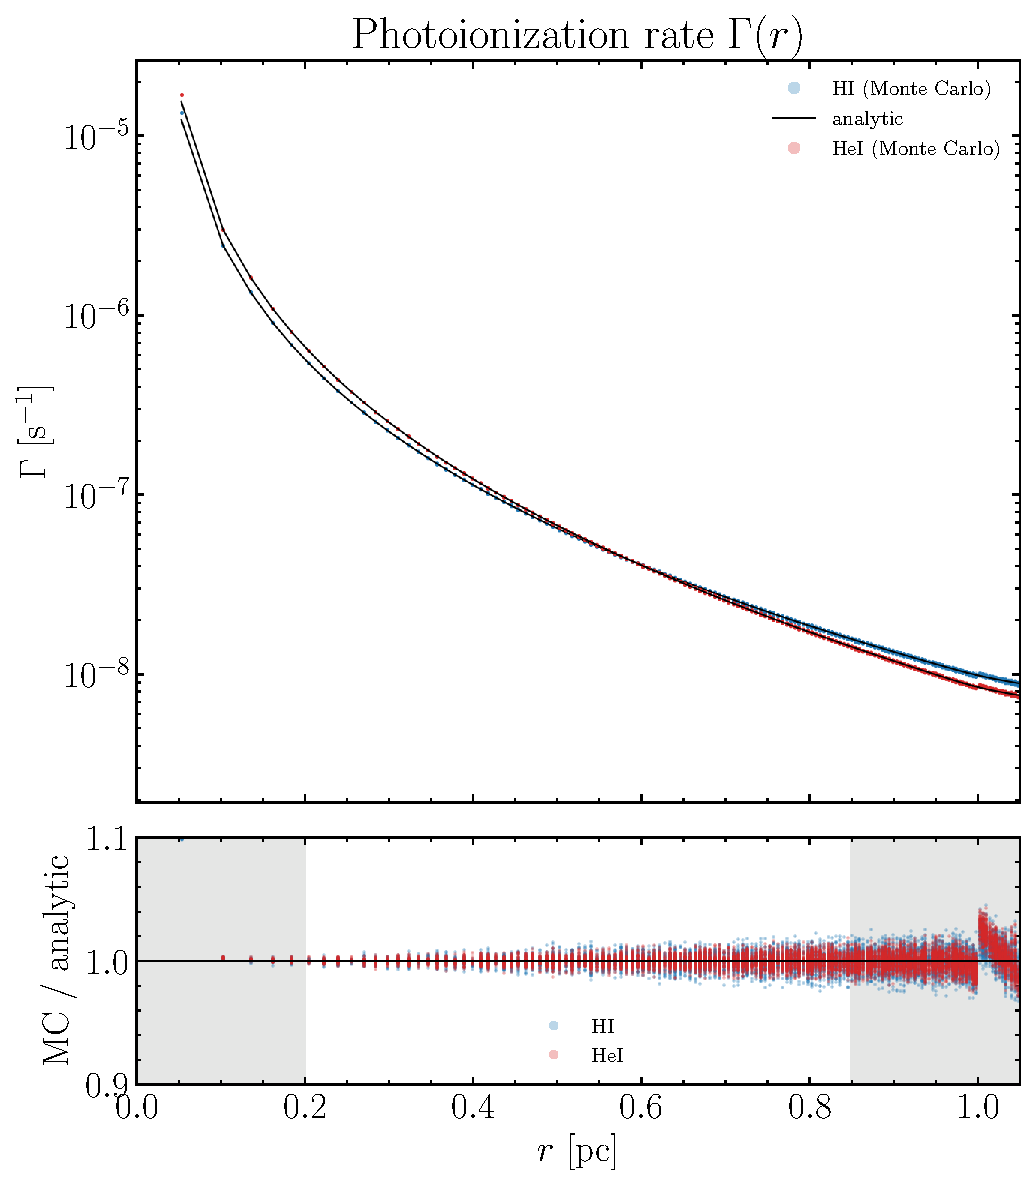
\includegraphics[width=\columnwidth]{figures/g0_gamma_check.pdf}
% source: tests/g0_gamma/g0_gamma_check.png (via docs/figures)
\caption{Rate-integral test: $\Gamma(r)$ from the Monte Carlo tally
(points) against the analytic point-source attenuation (lines); the lower
panel shows the ratio.  Shaded regions are excluded (cell-size effects at
the center, the voxelized sphere edge outside).}
\label{fig:g0}
\end{figure}

The Str\"omgren test uses a uniform $\nH = 100$ sphere, $\QH =
10^{49}\,\mathrm{s^{-1}}$ ($T_\star = 4\times10^4$~K), case B, and
$\Te = 10^4$~K.  For the reference we solve the spherically symmetric
ionization-equilibrium equations directly, with a deterministic radial
marching over $2\times10^4$ shells that carries the same band bins,
photoionization cross sections, and recombination and collisional rates as
the code: each bin's photon flux is attenuated with the running optical
depth evaluated at mid-shell, and the H/He ionization equilibrium is
solved shell by shell.
The sweeps must update opacities Gauss--Seidel style (a Jacobi sweep,
using the previous sweep's opacities, advances the front only one
absorption length in each pass); a few sweeps then converge.  ``Exact'' means
free of Monte Carlo noise and grid-converged at this resolution --- in
the sharp-edge limit it reproduces the analytic Str\"omgren radius
$R_S = [3\QH/(4\pi \nH^2 \alpha_B)]^{1/3} = 3.153$~pc, from which the
full solution differs physically (helium consumes photons; the front has
a finite width).  The 1D reference
gives an effective ionized radius $R_{\mathrm{eff}} = (3V_{\mathrm{ion}}/
4\pi)^{1/3} = 3.0243$~pc; a uniform level-7 octree gives 3.0448~pc
($+0.68\%$) and a level-6 one 3.0546~pc ($+1.00\%$), the difference being the
finite front width on a 0.147~pc cell against a front at 3.02~pc; a
front-refined octree with $3.5\times$ fewer cells
reproduces it to four decimals, while a center-refined control (coarsest
cells at the front) deviates by $+2.75\%$ --- the ionization front is the
one place needing resolution (Figure~\ref{fig:g1}).  With the thermal
balance on, $\Te(r)$ matches the 1D thermal reference to a median $0.77\%$
and a mean bias $+0.79\%$ (Figure~\ref{fig:g2a}).  Those figures are what the
comparison measures once the reference uses the run's own atomic data.  It
formerly carried the \citet{huignedin1997} case-B recombination coefficients
where the run uses the Badnell total with the Milne ground-level rate, a
frequency-averaged free-free Gaunt factor with no charge dependence where the run
separates $Z = 1$ from $Z = 2$, and \citet{verner1996} fits for H\,\textsc{i}
and He\,\textsc{ii} where the run uses the exact hydrogenic expression.  All
three are now taken from the code's own routines through a shared module that a
gate checks against the Fortran to machine precision.  Aligning the
recombination moved the median from $0.97\%$ to $0.77\%$; the Gaunt charge
dependence moved it $0.003$ percentage points, because a 40~kK blackbody leaves
almost no photons above 54.4~eV and the $Z = 2$ term is therefore negligible, and
the cross sections moved it $0.011$.  What is left is a property of the solution
rather than of the data.  Without metals the
metal-free nebula runs at 19--24~kK, the known overshoot that motivates the
trace-metal cooling.

\begin{figure*}[t]
\centering
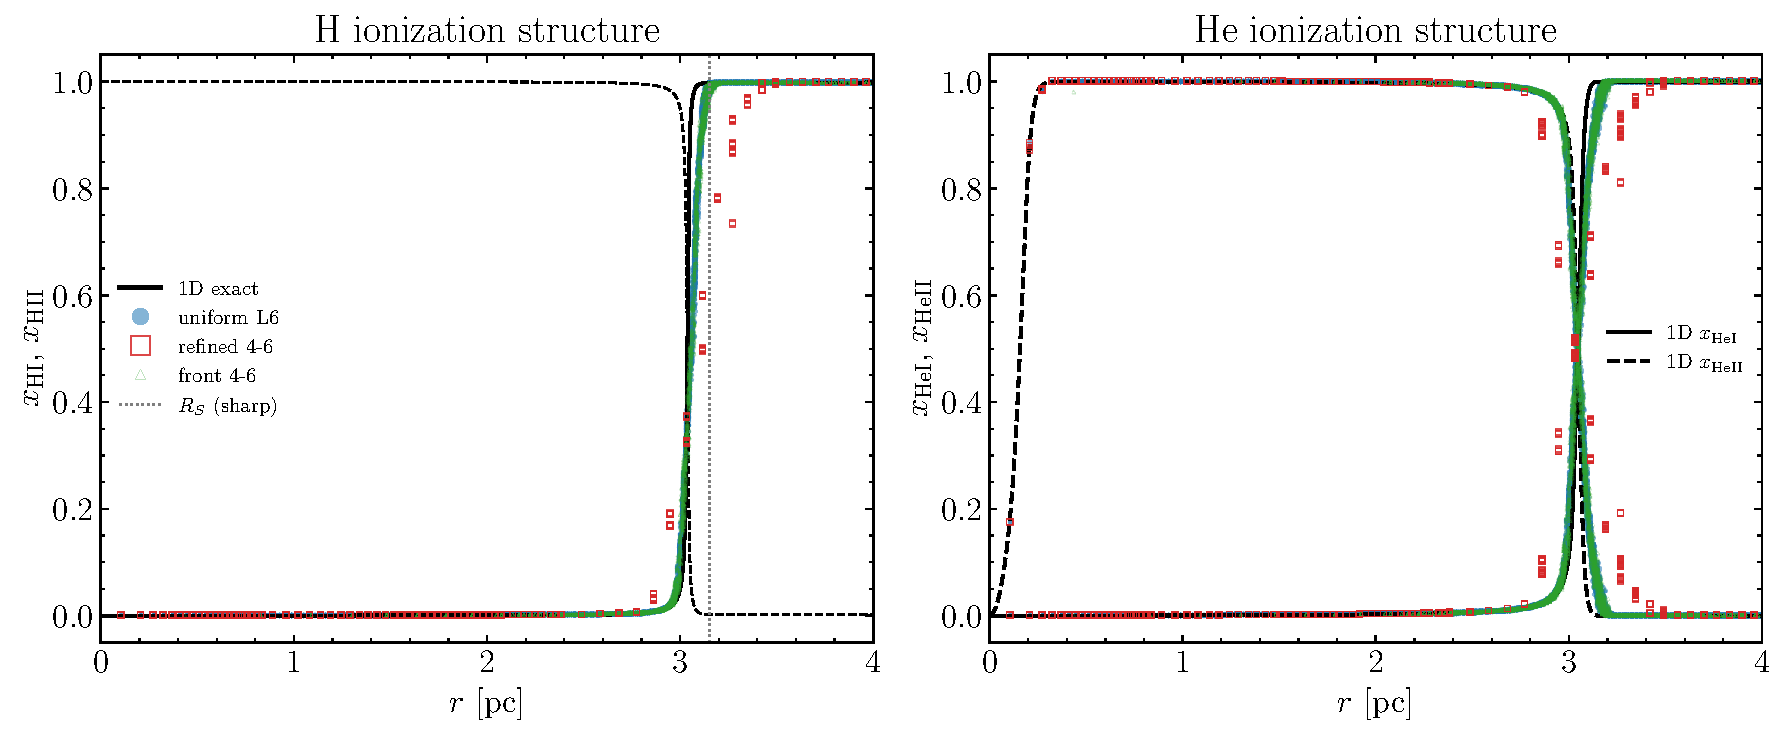
\includegraphics[width=0.9\textwidth]{figures/g1_stromgren_check.pdf}
% source: tests/g1_stromgren/g1_stromgren_check.png
\caption{Str\"omgren test: H and He ionization structure against the 1D
exact reference (black); uniform level-6 (blue), center-refined (red),
and front-refined (green, overlying blue).}
\label{fig:g1}
\end{figure*}

\begin{figure*}[t]
\centering
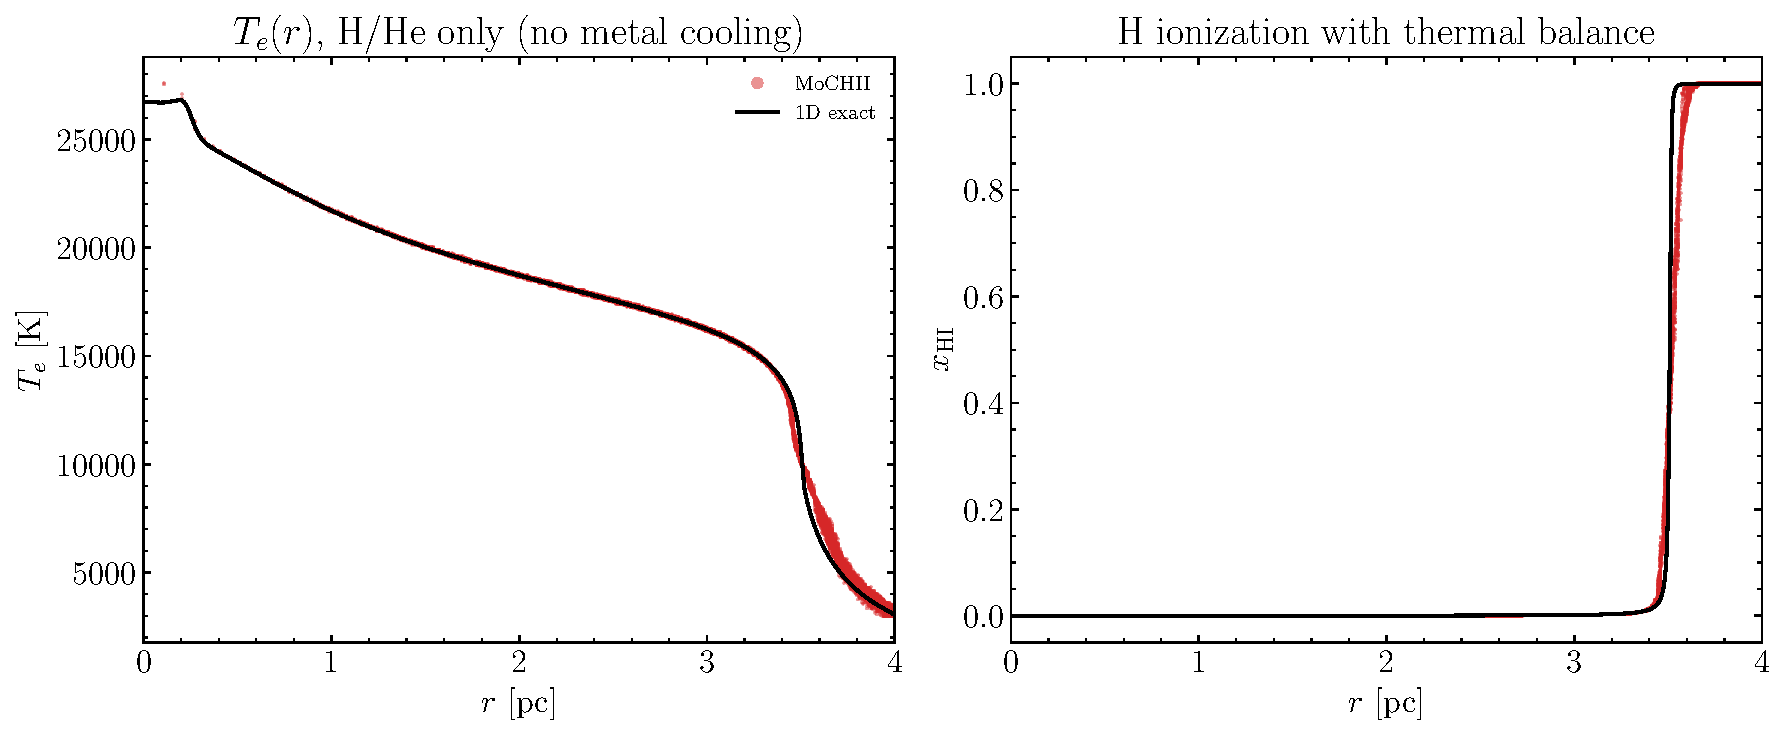
\includegraphics[width=0.9\textwidth]{figures/g2a_thermal_check.pdf}
% source: tests/g2a_thermal/g2a_thermal_check.png
\caption{Thermal test: $\Te(r)$ and $\xHI(r)$ with the thermal balance,
against the 1D exact reference.}
\label{fig:g2a}
\end{figure*}

\subsection{The Lexington benchmarks}
\label{sec:hii}

The HII20 and HII40 cases of the Lexington/Meudon comparison
\citep{ferland1995,pequignot2001} use 20 and 40~kK blackbody sources
($\QH = 1.0$ and $4.3\times10^{49}\,\mathrm{s^{-1}}$), $\nH = 100$ in a
hollow shell, and the standard Lexington abundances (He 0.1, C
$2.2\times10^{-4}$, N $4\times10^{-5}$, O $3.3\times10^{-4}$, Ne
$5\times10^{-5}$, S $9\times10^{-6}$).  They are the natural reference for a
new code because eight independent codes published results for the same two
models, so the benchmark carries its own measure of how large a
disagreement is significant.  Tables~\ref{tab:wood40} and~\ref{tab:wood20}
place \MoCHII{} next to those eight, in the compilation of
\citet{ercolano2003}, together with the Monte Carlo code of
\citet{wood2004} that was added to the same tables afterwards.

The \MoCHII{} runs compared here are configured to match the published
calculations wherever the setup is a choice rather than a physical
difference.  The ionizing luminosity is set from the benchmark blackbody
luminosity so that $\QH$ reproduces the specified $4.265\times10^{49}$
(HII40) and $1.004\times10^{49}\,\mathrm{s^{-1}}$ (HII20).  Stellar photon
energies are sampled continuously from the Planck spectrum with a Sobol
sequence, and every photoionization cross section is evaluated at the
sampled energy (Section~\ref{sec:band}); the 32-bin radiation array is only
a diagnostic tally.  The diffuse field is transported explicitly with
case-A rates and the \HeI{} channels
(Section~\ref{sec:diffuse}), the treatment the published codes use, so that
the comparison is not confounded by the transfer treatment.
The recombination-line emissivities
stay on the case-B tables, because the Lyman lines are optically thick in
these models whatever the continuum treatment is; the two cases are
separate switches (\code{par\%case\_ab} for the ionization,
\code{par\%line\_case} for the line tables).  The grid is a uniform level-6
octree ($64^3$ leaves) run with $2^{25}$ stellar packets (Sobol seed
20260728) to the volume-integrated convergence criterion.

We also ran \textsc{Cloudy} c25.00 \citep{cloudy2025} on both benchmarks and
carry it as the C25 column of the same two tables, providing a uniform
one-dimensional reference alongside the published multi-code spread.  Its
physics input is the
unmodified regression deck that \textsc{Cloudy} distributes for each case,
\code{tsuite/auto/hii\_paris.in} for HII40 and \code{hii\_coolstar.in} for
HII20 --- the same source, density, inner radius, and Lexington abundances as
above --- with only output commands appended; line luminosities are taken
from a \code{save line list absolute} file and divided by the \textsc{Cloudy}
H$\beta$ luminosity, and the averaged temperature is \textsc{Cloudy}'s own
$n_{\mathrm{e}}n_{\mathrm{p}}$-weighted volume average, the same weighting
used on both other sides.  The one geometric difference is that each deck
runs to its own stopping criterion rather than to a prescribed outer radius
--- an electron fraction of $10^{-2}$ at HII40, the 1000~K temperature floor
at HII20 --- so it carries a little more of the partly neutral edge than a
model truncated at $R_{\mathrm{out}}$ would.  The radii reached,
$1.467\times10^{19}$ and $8.97\times10^{18}$~cm, sit at the top of the
published $R_{\mathrm{out}}$ ranges (1.45--$1.47\times10^{19}$ and
8.7--$9.01\times10^{18}$~cm), so the two geometries are comparable, but the
low-ionization rows fed by that edge --- [O\,\textsc{i}], [S\,\textsc{ii}],
[N\,\textsc{ii}] --- are the ones where the difference could matter.

The temperature compared throughout this section is
$\langle T[N_{\mathrm{p}}N_{\mathrm{e}}]\rangle$, the electron temperature
averaged with the weight $n_{\mathrm{HII}}\nelec V$ --- the same definition
on both sides, evaluated leaf by leaf in \MoCHII{} and cell by cell in the
published models.  The inner-edge temperature $T_{\mathrm{inner}}$ that the
published tables also list is quoted separately where it is used.  Ionic
fractions are $\nelec V$-weighted means, the convention of MOCASSIN's own
output.  As a further point of comparison we also ran MOCASSIN 2.02 itself,
converged, on the HII40 model, and quote it below alongside the published
columns.

\emph{Ionization structure.}  The helium and metal ionization is sensitive
to the photon distribution around the \HeI{} edge.  A grouped spectrum can
assign all photons in a bin one representative energy and hence bias both
the threshold budget and the opacity.  The production calculations avoid
that approximation: they sample the Planck probability density continuously
and use the cross section at each sampled energy.  The resulting
$\langle\mathrm{He^{+}}\rangle/\langle\mathrm{H^{+}}\rangle$ is 0.712 at
HII40, below the published 0.715--0.829 (median 0.767) and C25's 0.741, and
0.047 at HII20, near the published median of 0.048 inside a spread of
0.034--0.077.

\emph{Temperature.}  The weighted temperature is 8169~K at HII40 and
6925~K at HII20.  Both match the \textsc{Cloudy} c25.00 solution of the
same two models --- 8210~K and 6910~K --- to $0.5\%$ and $0.2\%$, and both
lie above the 2000-era published ranges (7720--8199~K, median 8026, and
6402--6749~K, median 6662).  The inner-edge temperature is inside the
published spread at both, 7536~K at HII40 against a published 7370--8318~K
and 6938~K at HII20 against a published 6562--7224~K.  The converged
MOCASSIN 2.02 run of the HII40 model gives 8176~K, also inside the published
spread.  The two benchmark solutions therefore agree closely while remaining
within the range set by the independent calculations.

The temperature is set by the cooling treatment, and the two limits of that
treatment bracket the published set from opposite edges.  The
density-suppressed cooling used above --- the level populations at the local
$\nelec$, Section~\ref{sec:cooldata} --- gives the 8169 and 6925~K that
track \textsc{Cloudy}; the zero-density limit of the same fits, retained as
an option, overestimates the far-infrared line cooling at
$\nelec \sim 10^{2}\,\mathrm{cm^{-3}}$ and so places \MoCHII{} instead at
7894 and 6376~K, inside and just below the published ranges but $4$--$8\%$
below the two modern codes.  The offset between the two limits agrees in
sign and size with the far-infrared overestimate, which the next subsection
measures directly.

% Published columns: Tables 4 and 5 of Ercolano et al. (2003), transcribed
% and checked value by value against the paper.
% MoCHII column: continuous-energy production runs (Sobol seed 20260728,
% explicit diffuse field with the Milne ground continua, Q(H) matched to the
% specification, 2^25 packets, conv_crit='vol'); line entries are the L/L(Hbeta) column of
% results/continuous_energy/production/hii{40,20}_continuous_lines.txt
% (doublets summed), temperatures are from the matching rates files.
% C25 column: tests/cloudy_c25/, Cloudy c25.00 on the distributed decks.

\subsection{Cooling-budget verification at a fixed state}
\label{sec:coolcheck}

An emission-line comparison cannot by itself separate an error in the
atomic data from an error in the temperature, because each code's
temperature is the root of its own energy balance: too little cooling in
one channel raises $\Te$, which raises every other channel, and the
converged line ratios absorb part of the discrepancy.  The cooling data can
be compared free of that feedback only at a \emph{fixed} state.
\textsc{Cloudy} c25.00 writes such a decomposition --- its
\code{save cooling each} output lists the cooling rate of every ion and
every continuum channel zone by zone --- so the test is to take its
converged $(\Te, \nelec$, ionic fractions$)$ zone by zone, evaluate the
\MoCHII{} cooling terms on exactly that state, and integrate both over the
model volume.  What this measures is the absolute scale of two independent
atomic-data compilations, channel by channel, with nothing else in either
code entering.  It is the comparison that isolates the cooling data from
the temperature, which an equilibrium comparison cannot do, since the
latter shows only the temperature at which each code's own heating and
cooling cross.

On the HII40 model the two agree within the accuracy of the underlying
collision data.  With the $n$-level emissivities evaluated at the local
$\nelec$, the ratio \MoCHII/\textsc{Cloudy} is 1.02 for [O\,\textsc{iii}],
0.98 for [O\,\textsc{ii}], 1.00 for [S\,\textsc{iii}], 0.99 for
[N\,\textsc{ii}], 1.00 for [S\,\textsc{ii}], 1.00 for [Ne\,\textsc{ii}],
1.02 for [N\,\textsc{iii}], 1.02 for [S\,\textsc{iv}], 0.99 for
C\,\textsc{iii}], 0.94 for [C\,\textsc{ii}] and 0.99 for the \HI{}
collisional lines; summed over all line channels the two agree to $1.1\%$.
Two channels fall outside $\pm$10\%, [Ne\,\textsc{iii}] (1.30) and
[O\,\textsc{i}] (0.84), and they carry $1.9\%$ and $0.1\%$ of the budget.
The free-free continuum, an independent
check of the Gaunt factor and of the net ion charges entering it, agrees to
$0.2\%$.  Recombination cooling differs by bookkeeping rather than by data:
\textsc{Cloudy} reports the free-bound loss net of the escaping
recombination continuum, $4.02\times10^{37}\,\mathrm{erg\,s^{-1}}$, which
falls between the \MoCHII{} case-A and case-B sums ($6.61$ and
$3.62\times10^{37}$), the difference being the ground-state term that the
explicit diffuse field re-emits instead of losing.  The heating side of the
same \textsc{Cloudy} model balances its cooling to $1.3\times10^{-4}$ and
deposits 4.57~eV for each ionizing photon, so the comparison state is
itself an equilibrium one.

The same $n$-level emissivities at the local $\nelec$ are what the thermal
loop uses by default (Section~\ref{sec:cooldata}), so this fixed-state
agreement is the cooling the converged benchmark carries.  Replacing them
by the zero-density limit of the same fits (Eq.~\ref{eq:cool}, the
\code{cooling\_model = low\_density} option) raises the summed line cooling
to $1.116$ times \textsc{Cloudy}'s.  The excess is not spread over the
ions: it is 5.1 percentage points of the line budget in [O\,\textsc{iii}]
and 3.9 in [C\,\textsc{ii}], and in both it sits entirely in the
far-infrared fine-structure lines, whose critical densities are at or below
the local $\nelec = 110\,\mathrm{cm^{-3}}$.  Since the line channels carry
$79\%$ of the cooling budget, that is a $9\%$ excess in the total, and it
accounts for the temperature difference quantitatively: scaling $\Te$ on the
fixed state until the \MoCHII{} zero-density terms radiate the same total
power --- \textsc{Cloudy} balances its own heating at the unscaled
temperature, and the photoheating of the two codes agrees --- gives 7784~K
against \textsc{Cloudy}'s 8210~K, close to the 7894~K the converged
zero-density run reaches.  Removing the overestimate, the density-suppressed
default reaches 8169~K, matching \textsc{Cloudy} to $0.5\%$
(Section~\ref{sec:hii}).  The far-infrared overestimate, not the atomic
data, is thus what separates the two limits, and the $(\Te,\nelec)$ table of
Section~\ref{sec:cooldata} removes it.

\emph{Sensitivity to the other ingredients.}  The remaining modeling
choices are smaller levers than the cooling function, and each is measured
by an in-code experiment.  The transport treatment is the largest of them:
replacing the case-A explicit diffuse field by the case-B on-the-spot
approximation, with every other setting fixed, gives 7898~K at HII40 and
6899~K at HII20, so the explicit field used here raises $\Te$ by $4.0\%$
and $1.8\%$ and moves the two benchmarks the same way.  Substituting
MOCASSIN-style recombination
(P\'equignot 1991 radiative plus Nussbaumer--Storey 1983 dielectronic) for
the Badnell 2023 data, whose $\alpha(\mathrm{X\,\textsc{iii}} \to
\mathrm{X\,\textsc{ii}})$ are systematically lower (ratios 0.72--0.84),
moves $\Te$ by $0.15\%$ and the carbon, nitrogen and oxygen ionization
fractions by about 0.02, so the recombination vintage is a minor lever on
both.  The dominant
[O\,\textsc{iii}] collision strengths are stable across database
generations: the $^3\mathrm{P}$--$^1\mathrm{D}$ effective collision
strength is 2.283 in the CHIANTI~v7 compilation behind the published
MOCASSIN column and 2.262 in v11 at $10^4$~K, a $0.9\%$ difference worth
less than 30~K.  The photoionization heating is standard, with mean
photoelectron energies $\langle h\nu - 13.6\rangle_{\mathrm{H}} = 3.9$~eV
and $\langle h\nu - 24.6\rangle_{\mathrm{He}} = 4.1$~eV.  Grid resolution
is treated separately below.

\emph{Line ratios.}  The line intensities follow from that temperature and
ionization structure rather than from the emission calculation, which is
exact to the accuracy of its input data (Section~\ref{sec:cooldata}: the
$n$-level solver reproduces an independent reference solver to four digits,
and the fitted collision data reproduce direct CHIANTI evaluations to
0.05--0.5\%).  At HII40 the infrared fine-structure lines, whose excitation
energies are small enough that they are nearly temperature-independent, sit
with the published set ([Ne\,\textsc{iii}] 15.5\,$\mu$m 0.283 in a
published 0.263--0.429; [Ne\,\textsc{ii}] 12.8\,$\mu$m 0.206 in
0.177--0.217; [O\,\textsc{iii}] 52+88\,$\mu$m 2.43 just above 2.10--2.42),
and so do the temperature-sensitive optical lines of the same ion:
[O\,\textsc{iii}] 5007+4959 is 2.36 against a published 1.64--3.27, and the
auroral [O\,\textsc{iii}] 4363, the most temperature-sensitive entry in the
tables, is 0.0044 against a published 0.0022--0.0070.  The lines that fall
outside the published ranges are examined below.

\emph{H$\beta$ and the photon budget.}  A recombination line is a photon
counter, and $L(\mathrm{H}\beta)$ therefore tests whether the model is
radiation-bounded: every ionizing photon absorbed by hydrogen returns as a
recombination, and a fixed fraction of those recombinations produces
H$\beta$.  Both models here are bounded.  At HII40 the ionization front is
captured inside the prescribed sphere, at $1.45\times10^{19}$~cm against an
outer radius of $1.46\times10^{19}$~cm, and the outermost shell is $57\%$
neutral; at HII20 the outer shells are fully neutral.  The budget closes
accordingly: summing the case-B recombinations over the converged solutions
gives $0.950\,\QH$ and $0.970\,\QH$.  What hydrogen does not absorb is
taken up by helium, which at HII40 absorbs $0.112\,\QH$ and returns most of
it to hydrogen through the \HeI{} diffuse channels.  The predicted
$L(\mathrm{H}\beta) = 1.93\times10^{37}$ and
$4.68\times10^{36}\,\mathrm{erg\,s^{-1}}$ are $4$--$6\%$ below the
published medians (some $3$--$4\%$ below the lowest published values),
consistent with the $5.0\%$ and $3.0\%$ of $\QH$ that the recombination
budget assigns to helium rather than to hydrogen, together with the weak
temperature dependence of the effective H$\beta$ emissivity at the higher
benchmark temperature.  The absolute H$\beta$ luminosity is thus set by the
recombination budget, and adds no discrepancy of its own.

\emph{The complete published line list.}  The full benchmark line lists,
with all published codes, a \textsc{Cloudy}~c25.00 column, and the
\MoCHII{} column, are given in Appendix~\ref{app:lines}
(Tables~\ref{tab:wood40} and~\ref{tab:wood20}); they repeat the comparison
over the full benchmark line list in
the form used by \citet{wood2004}, whose Tables 1 and 2 add their own Monte
Carlo code (WME) to the eight other codes of the comparison; the
\MoCHII{} and C25 columns provide two additional reference solutions.  The
low-ionization edge line [O\,\textsc{i}]
6300+6363 is 0.0169 at HII40, above the published 0.0059--0.012 range; it is
particularly sensitive to the thin partly neutral edge.  The complete
comparison is given directly in the tables.

The C25 column provides a uniform reference, and with the two temperatures
matched the line
ratios track C25 across the board.  At HII40, where the weighted temperature
equals C25's, both the temperature-insensitive far-infrared lines and the
temperature-sensitive optical and auroral lines agree with C25 to a few
percent: among the infrared lines [O\,\textsc{iii}] 52+88\,$\mu$m is
$1.01\times$ C25, [N\,\textsc{iii}] 57.3\,$\mu$m $1.01\times$ and
[S\,\textsc{iii}] 18.7\,$\mu$m $1.01\times$; among the optical ones
[O\,\textsc{iii}] 5007+4959 is $0.96\times$, its auroral 4363 $0.94\times$
and [O\,\textsc{ii}] 3726+3729 $0.98\times$ --- the same optical and auroral
lines that the zero-density cooling, running $3.8\%$ cooler, had suppressed
to $0.72$--$0.84\times$.  That the temperature-sensitive lines fall into
line with C25 exactly when the temperature does is the line-level
counterpart of the cooling match.  At HII20, where \MoCHII{} is $0.2\%$
hotter than C25, [O\,\textsc{ii}] 3726+3729 is $1.01\times$ C25.  The
residual outliers at HII40 are not temperature: [Ne\,\textsc{iii}]
15.5\,$\mu$m ($1.32\times$) and 3869+3968 ($1.22\times$),
[O\,\textsc{i}] 6300+6363 ($1.55\times$, on a line the thin neutral edge and
the grid resolution govern), and C\,\textsc{iii}] 1907+1909 ($0.89\times$),
each an ionization or collision-strength difference in a single ion.

The C25 and published columns illustrate the benchmark's code-to-code
spread.  [S\,\textsc{ii}] 6716+6731 at
HII40 is the clearest case: the GF entry is 0.137, C25 gives 0.304 and
\MoCHII{} 0.320; the two latter values differ by $5\%$.  Sulfur at HII20 is
the same story in the other direction: [S\,\textsc{iii}] 18.7\,$\mu$m
(0.216 against a published 0.34--0.46) and [S\,\textsc{iii}] 9532+9069
(0.304 against 0.465--0.604) fall \emph{below} every published code, and so
does C25 (0.209 and 0.293), while [S\,\textsc{ii}] 6716+6731 sits inside the
published range for both (0.780 and 0.744).  Both C25 and \MoCHII{} have the
same S\,\textsc{ii}/S\,\textsc{iii} ordering, which points at the sulfur
data rather than at either code.  A band experiment bounds one further
difference: \textsc{Cloudy} carries the full stellar spectrum, so photons
below 13.6~eV ionize S$^{0}$ (10.36~eV) and C$^{0}$ (11.26~eV) in the
partly neutral edge, while the benchmark band here starts at the hydrogen
edge.  Extending the \MoCHII{} band down to 6~eV raises
[S\,\textsc{ii}] 6716+6731 by 6\% at HII20 and by under 1\% at HII40, with
the other low-ionization lines moving by at most a few percent --- a real
ingredient of the low-ionization rows, but far too small to account for the
[S\,\textsc{iii}] difference.

A second, structural difference is worth naming here, because it affects
sulfur specifically.  The published columns are not all built on the same
set of ionization stages: the code of \citet{wood2004}, and
\textsc{CMacIonize} after it, omit neutral sulfur and start the sulfur
chain at S$^{+}$, so that in gas where the ionizing field has been absorbed
all sulfur is S$^{+}$ by construction; oxygen and neon in the same codes do
carry their neutral stages.  \textsc{Mocassin} instead solves the neutral
stage of every element as an unknown, as \MoCHII{} and \textsc{Cloudy} do.
The convention matters only outside the ionization front, where it fixes
the S$^{+}$ reservoir that feeds [S\,\textsc{ii}] rather than letting it
recombine to S$^{0}$; it is one of the ingredients of the scatter among the
published sulfur entries, and it is worth keeping in view when a single
[S\,\textsc{ii}] ratio is used to judge a code.

\emph{Radial structure.}  Figures~\ref{fig:wood40} and \ref{fig:wood20}
give the radial ionization and temperature structure in the panel layout of
\citet{wood2004}, their Figures 1 and 2, so that the two can be read panel
by panel.  The morphology is the published one throughout.  At HII40 the
hydrogen and helium neutral fractions rise monotonically from
$4\times10^{-5}$ and $2\times10^{-4}$ at the inner edge, the singly and
doubly ionized fractions of carbon, nitrogen and oxygen cross within
0.15~pc of one another near 4.0~pc, C$^{+3}$ peaks at $0.05$ and is
confined to the inner region, and the temperature falls slightly out to
about 2.2~pc before climbing steeply toward the front.  At HII20 helium is
essentially all neutral beyond
1.3~pc while hydrogen stays ionized out to 2.9~pc, so the doubly ionized
metals occupy only a thin inner shell.  Both models are radiation-bounded,
so both outer radii are predictions.  The ionized-volume-equivalent radius
$(3V_{\mathrm{ion}}/4\pi)^{1/3}$ and the shell-averaged
$x_{\mathrm{HII}} = 0.5$ crossing that the tables carry as
$R_{\mathrm{out}}$ are $1.441$ and $1.447\times10^{19}$~cm at HII40 against
a published 1.45--$1.47\times10^{19}$, and $8.80$ and
$8.91\times10^{18}$~cm at HII20 against a published
8.7--$9.01\times10^{18}$: the two definitions of the outer boundary are not
identical, but they locate the same front, and both fall inside the
published range at HII20 and within $0.6\%$ of its lower end at HII40,
consistent with a recombination budget of $0.95$--$0.97\,\QH$.  The temperature panels
reproduce the published shape --- a shallow inward decline followed by a
steep rise at the front, where the surviving radiation field is hardest.

\emph{Grid resolution.}  The two three-dimensional codes of the comparison
state what they used, and it is worth placing \MoCHII{} beside them, because
a Monte Carlo photoionization calculation on a Cartesian grid has a
resolution as well as a photon budget.  \citet{ercolano2003} ran the
published \textsc{Mocassin} benchmark columns on $13\times13\times13$ cells
with the source in a \emph{corner}, so that the grid covers one octant of the
spherically symmetric model; in their words, ``although the number of
sampling points along each orthogonal axis is only 13, this is the
equivalent of a one-dimensional code with 273 radial points.''
\citet{wood2004} used $65^3$ cells over the full box with the star at the
center, which they describe as matching a $33^3$ \textsc{Mocassin} octant,
i.e.\ a cell width of ``3\% of the radius,'' and $10^8$ photon packets.  The
\MoCHII{} runs here use a uniform level-6 octree, $64^3 = 262\,144$ leaves
over the full box with the source at the center, and $2^{25}$ packets.
\MoCHII{} and \citet{wood2004} are therefore at essentially the same
resolution --- $4.6\times10^{17}$ against $4.4\times10^{17}$~cm on a side at
HII40 --- and both are about $2.5\times$ finer per axis than the octant grid
behind the published \textsc{Mocassin} column.  We did not repeat the
benchmark on a deliberately coarsened grid, because the quantity at issue is
already resolution-converged in the direction that matters: the front
re-refinement test of Section~\ref{sec:refine} shows $R_{\mathrm{eff}}$
changing by $+0.008\%$ between a native level-7 grid and a coarser
re-refined equivalent, and \citet{ercolano2003} themselves attribute to grid
coarseness only their inner-edge temperature $T_{\mathrm{inner}}$ --- which
their coarse cells make too \emph{low}, since a cell carries the temperature
of its center rather than of the illuminated face --- and not
$\langle T[N_{\mathrm{p}}N_{\mathrm{e}}]\rangle$ or the line ratios compared
here.  Grid resolution is thus not a candidate for the differences discussed
above, with the exception of the thin partly neutral edge that feeds
[O\,\textsc{i}] 6300+6363, which one cell width does not resolve in any of
the three-dimensional codes.

The radial ionization and temperature structure of both benchmarks is
shown in Appendix~\ref{app:lines} (Figures~\ref{fig:wood40} and
\ref{fig:wood20}), in the panel layout of \citet{wood2004}.


\emph{Reference-code context.}  The C25 and GF columns demonstrate the
intrinsic spread among implementations and atomic-data choices.  For example,
at HII40 [S\,\textsc{ii}] 6716+6731 is 0.304 (C25) and 0.137 (GF), while
[O\,\textsc{iii}] 4363 is 0.0046 and 0.00235.  At HII20 the two
[S\,\textsc{iii}] entries are 0.209 and 0.293 in C25, compared with 0.445
and 0.501 in GF.  The published spread and the independently calculated C25
column therefore provide more informative reference ranges than any single
column.

\emph{Where \MoCHII{} sits among the codes.}  \citet{pequignot2001} and
\citet{ercolano2003} note that the eight codes do not scatter randomly:
GF, HN, and DP agree more tightly with one another --- and, in the
planetary-nebula cases, with \textsc{Mocassin} --- than with TK, PH, and RS,
a coherence they attribute to more recently updated atomic data and to a
more careful treatment of the diffuse radiation field.  A second grouping
runs along the transfer treatment: the codes that solve the transfer exactly
(RR, PH, and \textsc{Mocassin}) give systematically lower temperatures at
the illuminated inner edge, because the radiation field there is softer than
an approximate treatment makes it.  \MoCHII{} belongs with the first group on
the data axis --- exact hydrogenic and Verner cross sections, Badnell 2023
recombination, CHIANTI v11 collision strengths, the same vintage
\textsc{Cloudy} uses --- and with the second on the transfer axis, since the
analytic direct-field estimator and the explicit diffuse field used for
these benchmarks are an exact treatment in three dimensions; its inner-edge
temperature is correspondingly in the lower half of the published
$T_{\mathrm{inner}}$ range.  Its ionization structure, its outer radius,
its H$\beta$ luminosity and most of its line ratios land inside the
published spread, with helium at the low edge of it in the same direction
as \textsc{Cloudy} c25.00, and its weighted temperature matches that
solution to $0.5\%$ at HII40 and $0.2\%$ at HII20.  The cooling treatment that
achieves this, the density suppression of Section~\ref{sec:cooldata}, is
what separates it from the zero-density limit that leaves both benchmarks
$4$--$8\%$ cooler; the fixed-state comparison quantifies the offset between
the two and shows it to be a property of the cooling function, not of the
atomic data.

%==========================================================================
\section{Solution-driven front refinement}
\label{sec:refine}

A distinguishing capability of the octree grid is that the refinement can
be driven by the ionization solution itself.  At a chosen iteration the
octree is rebuilt: a leaf is flagged as ``front'' when
$\epsilon < \xHI < 1-\epsilon$ or a face neighbor differs by more than a
threshold; the new tree carries the maximum level wherever a cell overlaps
a front-flagged leaf and a base level elsewhere.  The gas state and opacity
map over by position, and every dependent array is recreated.  All ranks
rebuild identically from the shared state, and the old grid's
shared-memory windows are freed immediately after the position sampling, so
repeated re-refinement neither leaks nor holds two grids in memory at
once.

On the Str\"omgren configuration, starting at level 5 and rebuilding to
level 7 at iteration 15 (32\,768 $\to$ 464\,311 leaves), the re-refined
grid gives $R_{\mathrm{eff}} = 3.0432$~pc against a native uniform level-7
grid's 3.0430~pc (2\,097\,152 leaves) --- agreement to $+0.008\%$ with
$4.5\times$ fewer cells, and both improve on level 6 ($+1.00\%$), as
resolution convergence expects (Figure~\ref{fig:g4refine}).  The front
profiles overlie exactly.

\begin{figure}[t]
\centering
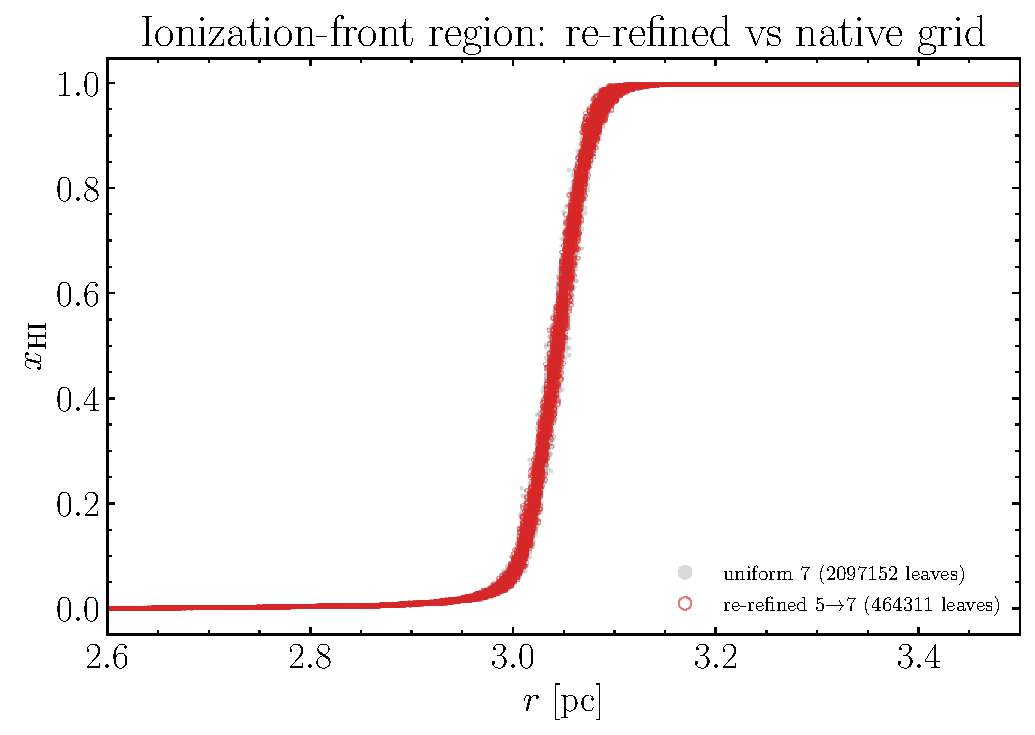
\includegraphics[width=\columnwidth]{figures/g4_refine_check.pdf}
% source: tests/g4_refine/g4_refine_check.png
\caption{Re-refinement test: the front profiles of the re-refined
$5\to7$ octree and the native uniform level-7 grid overlie exactly, at
$4.5\times$ fewer cells.}
\label{fig:g4refine}
\end{figure}

As a demonstration on a realistic geometry, \MoCHII{} was run on an
Illustris-TNG 60-kpc cutout (density and neutral-fraction columns from the
simulation), with a $\QH = 10^{53}\,\mathrm{s^{-1}}$, 40-kK source at the
density peak and thermal balance, metals, and re-refinement enabled
(Figure~\ref{fig:tng}).  Dense clumps cast sharp neutral shadows, the
circumgalactic gas sits at $\xHI \sim 10^{-4}$ with an $\nelec$-weighted mean
$\Te = 7502$~K, and the refinement (32\,768 $\to$ 617\,135 leaves) tracks
the \emph{distributed} ionization topology of a turbulent medium --- clump
skins and partially ionized gas rather than a single thin shell.  This is
the regime for which the volume-integrated convergence criterion
(Section~\ref{sec:iterate}) was designed.

\begin{figure*}[t]
\centering
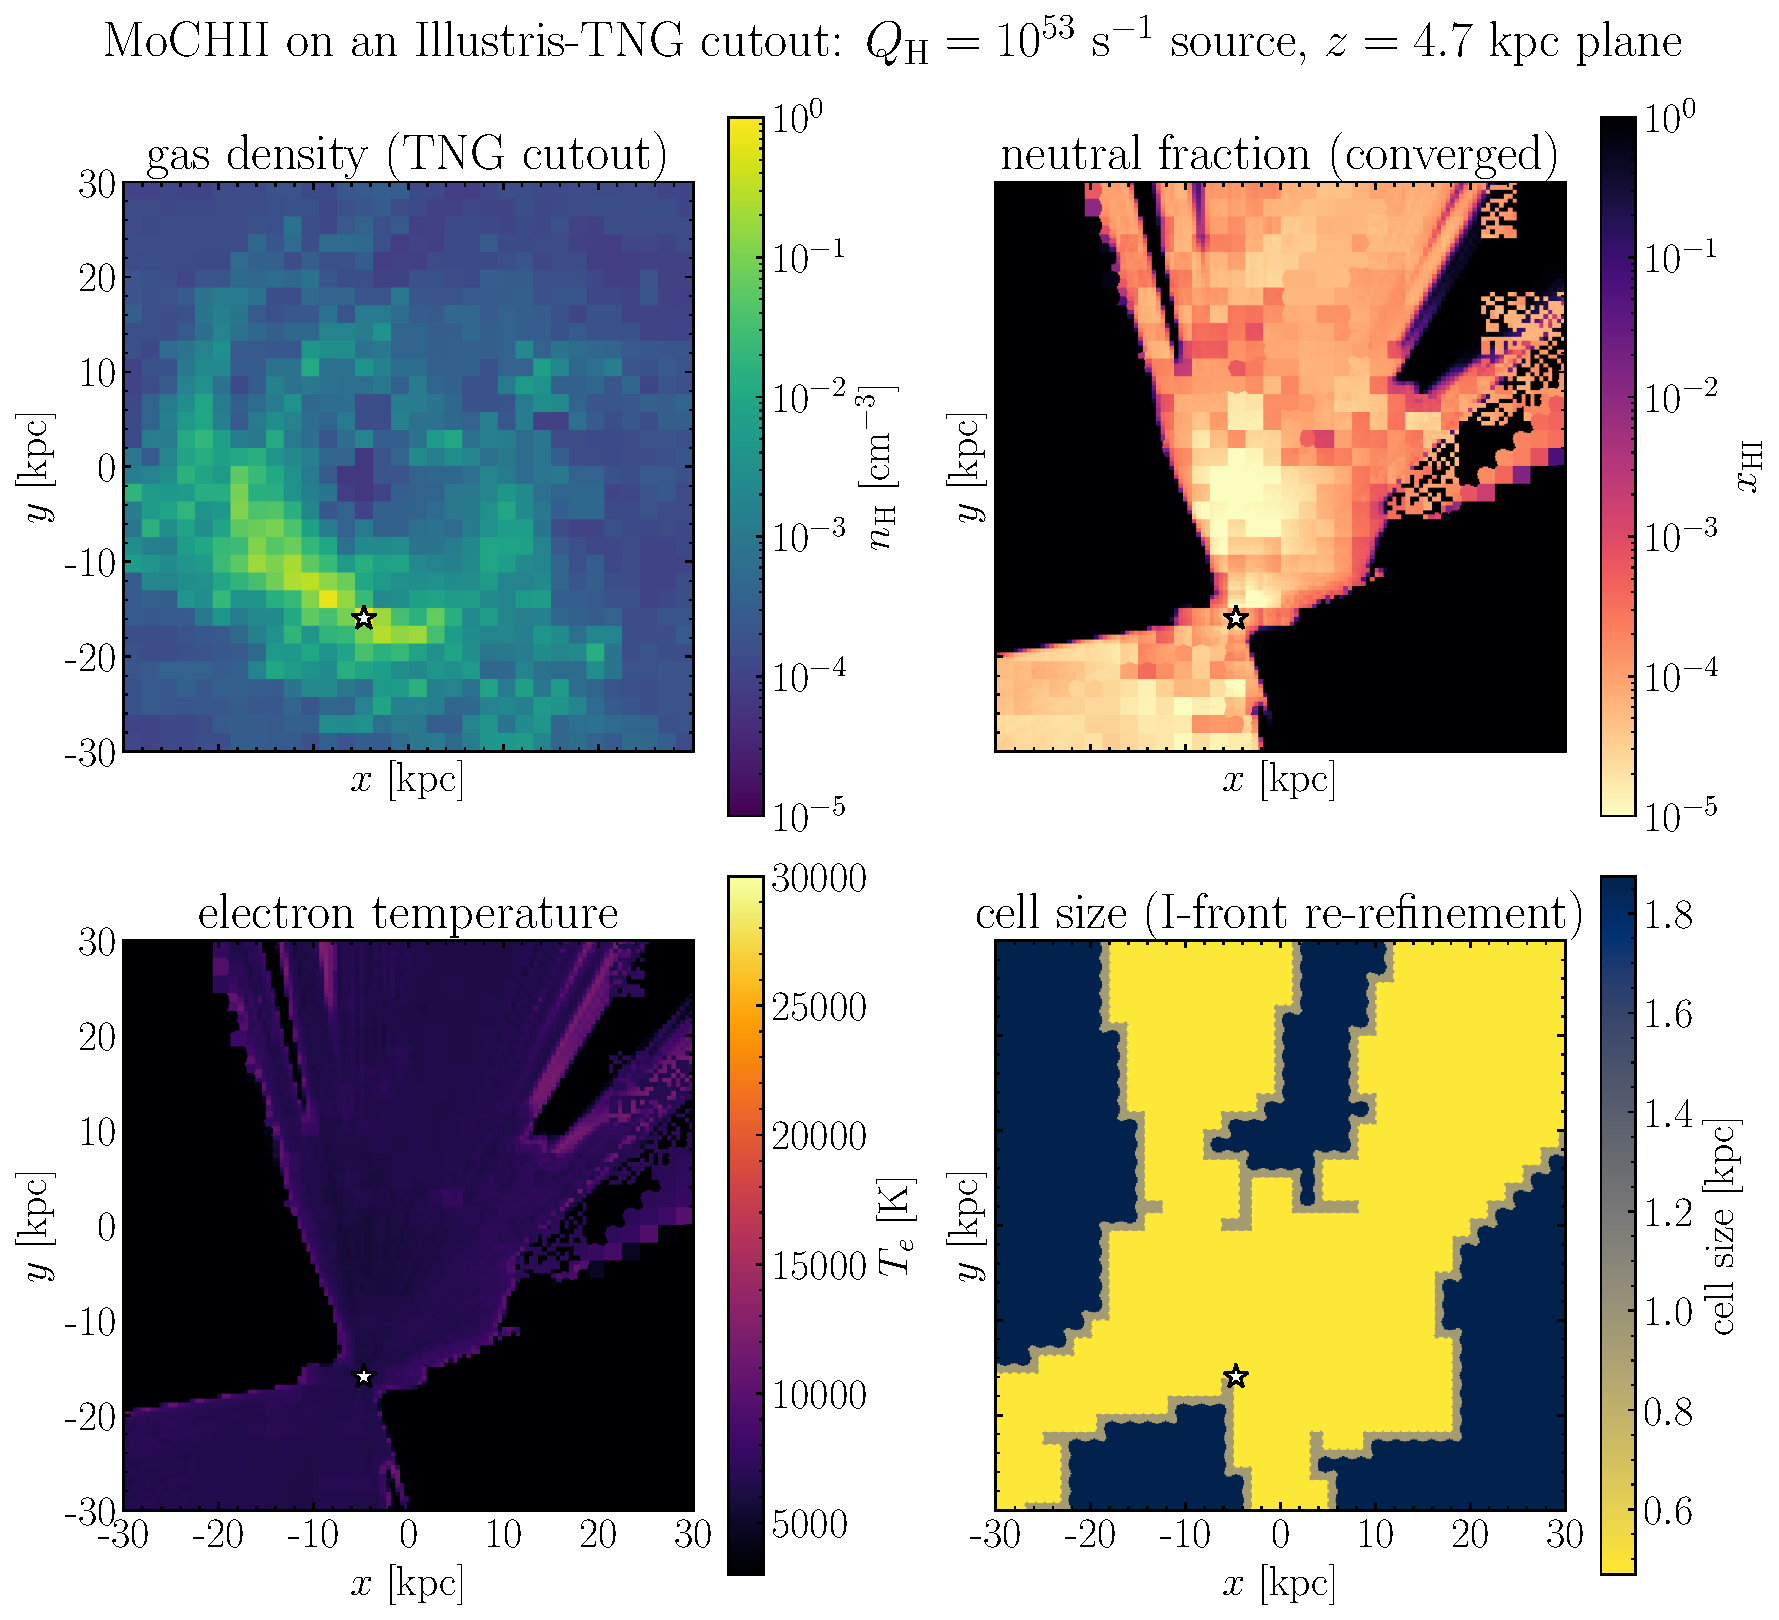
\includegraphics[width=0.7\textwidth]{figures/g4_tng_maps.pdf}
% source: tests/g4_tng/g4_tng_maps.png
\caption{\MoCHII{} on an Illustris-TNG cutout: gas density, converged
neutral fraction (note the clump shadows), electron temperature, and the
re-refined cell size, in the source plane.}
\label{fig:tng}
\end{figure*}

%==========================================================================
\section{Dust and PAH coupling}
\label{sec:dust}

Because \MoCHII{} is built on a dust radiative-transfer engine, the dust
physics is a first-class part of the transport.  The coupling has four
parts.

\emph{Absorption competition.}  Each band bin adds a dust absorption
opacity $\kappa_{\mathrm{d}} = \rho\kappa\,s_{\mathrm{abs}}(b)$ with
$s_{\mathrm{abs}}(b) = (1-a(E_b))\,C_{\mathrm{ext}}(E_b)/
C_{\mathrm{ext}}(\lambda_{\mathrm{ref}})$ from a WD01/D03 $R_V = 3.1$
extinction table \citep{weingartner2001,draine2003} covering the EUV, where
$C_{\mathrm{abs}}/\mathrm{H} = 1.75\times10^{-21}$ at 13.6~eV falls to
$3.96\times10^{-22}\,\mathrm{cm^2}$ at 100~eV.  On the dusty Str\"omgren
test, against a 1D reference carrying identical dust absorption, the full
MW dust gives $R_{\mathrm{eff}} = 2.205$~pc versus the reference 2.191~pc
($+0.66\%$), reproducing the classic dusty reduction $R/R_0 = 0.722$
(Figure~\ref{fig:duststrom}); dust absorbs $\sim$60\% of the band luminosity
there.

\emph{Scattering.}  With scattering enabled the scattering opacity joins
the extinction (in-band Henyey--Greenstein asymmetry $g = 0.67$--$0.99$,
strongly forward), and interactions are sampled by a forced-first-flight
scheme after the analytic direct walk, with an albedo weight at each
interaction and Russian roulette.  The full-scattering Str\"omgren radius,
2.196~pc, is within $0.4\%$ of the absorption-only 2.205~pc: the in-band
dust is strongly forward-throwing, so a scattered photon is barely deflected
and scattering acts almost as pure transmission, exactly as expected.

\emph{Live ionization-dependent dust with a PAH split.}  Following
\citet{laursen2009}, the dust content is traced by the metallicity-scaled
hydrogen, with neutral gas carrying the full dust column and ionized gas
only a survival fraction $f_{\mathrm{ion}}$ of it (grains are eroded where
the hydrogen is ionized).  \MoCHII{} evaluates this on the \emph{computed}
neutral fraction and refreshes it every iteration, and it splits the grains
into a large-grain share $1 - f_{\mathrm{PAH}}$ and a PAH share
$f_{\mathrm{PAH}}$ with independent ionized-gas survival, so the dust
opacity of a leaf is
\begin{multline}
  \kappa_{\mathrm{d}} \propto \frac{Z}{Z_{\mathrm{ref}}}\,\nH
  \big[(1 - f_{\mathrm{PAH}})(\xHI + f_{\mathrm{ion}}\,x_{\mathrm{HII}}) \\
  + f_{\mathrm{PAH}}(\xHI + f_{\mathrm{ion,PAH}}\,x_{\mathrm{HII}})\big],
\end{multline}%
with $x_{\mathrm{HII}} = 1 - \xHI$ and $f_{\mathrm{ion,PAH}} = 0$ by
default (PAHs destroyed in ionized gas).  Because this dust opacity is
rebuilt from the ionization state each iteration while that state is in
turn set by the dust-attenuated field, the dust--ionization feedback loop
is solved self-consistently; it converges to a near dust-free interior
($R/R_0 = 0.996$).

Figure~\ref{fig:duststrom} contrasts the three treatments on the same
Str\"omgren configuration.  Static full MW dust competes with hydrogen for
the ionizing photons throughout the volume, so the ionization front is
pushed inward to $R_{\mathrm{eff}} = 2.21$~pc, the classic dust-limited
size ($R/R_0 = 0.722$).  Under \code{laursen09\_live}, by contrast, the
interior dust vanishes together with the neutral fraction it is tied to ---
once the gas is ionized it carries essentially no dust to absorb the
ionizing field --- so the front profile overlies the dust-free case almost
exactly ($R_{\mathrm{eff}} = 3.04$~pc, $R/R_0 = 0.996$).  The physical
distinction is that only the neutral gas beyond the front and its thin skin
retain dust, which is where the dust column that matters for the escaping
radiation actually sits.

\begin{figure}[t]
\centering
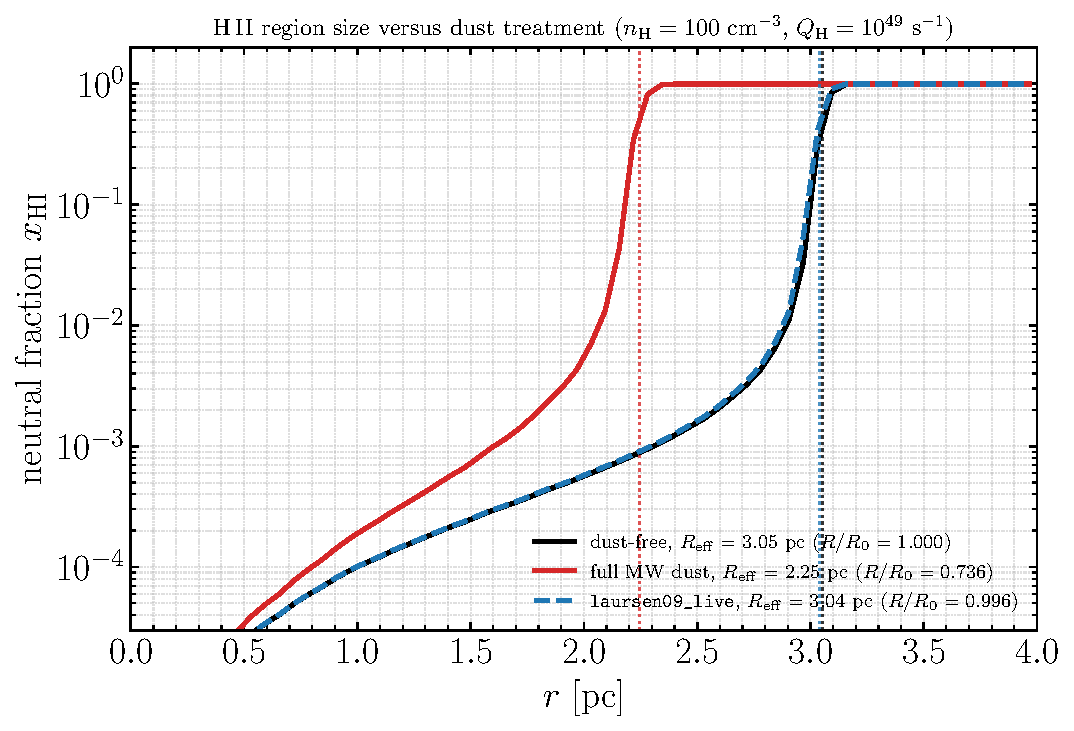
\includegraphics[width=\columnwidth]{figures/dust_stromgren.pdf}
% source: figures/make_dust_stromgren.py, from
%   tests/g1_stromgren/g1_stromgren_rates.h5 (dust-free),
%   tests/d_dusty/d_dust_full_rates.h5 (full MW dust),
%   tests/d_dusty/d_dust_l09_rates.h5 (laursen09_live).
\caption{H\,\textsc{ii} region size versus dust treatment: the radial
neutral-fraction profile $\xHI(r)$ for the dust-free, full MW dust, and
\code{laursen09\_live} runs of the same Str\"omgren configuration
($\nH = 100\,\mathrm{cm^{-3}}$, $\QH = 10^{49}\,\mathrm{s^{-1}}$,
$T_\star = 4\times10^4$~K, case B).  Dotted vertical lines mark each
effective ionized radius $R_{\mathrm{eff}}$.  Full MW dust pushes the
ionization front inward to $R/R_0 = 0.722$, while the live
ionization-dependent dust vanishes in the ionized interior and recovers the
dust-free size ($R/R_0 = 0.996$).}
\label{fig:duststrom}
\end{figure}

\emph{Grain heating, equilibrium temperature, and IR emission.}  The
transported grain heating drives the equilibrium dust temperature by
balancing the absorbed power against $4\pi\int s_{\mathrm{abs}}(\nu)
B_\nu(T)\,d\nu$; with the band widened to 6~eV, $T_{\mathrm{d}}$ runs from
87~K at 0.3~pc to 28~K at the sphere edge (the canonical \HII-region
gradient), and the IR spectrum integral closes on the absorbed power to
$L_{\mathrm{IR}}/L_{\mathrm{abs}} = 1.000$.  A full stochastic dust
emission solve (the \MoCafe{} SEDust module; astrodust, DL07, and Zubko
grain models with PAH bands, after \citealt{drainel12007}) is available at
output time: it uses the size-resolved stochastic-heating spectrum as a
\emph{shape} normalized to the transported absorbed power, so the
normalization is exact by construction.  With the live PAH share
(Figure~\ref{fig:pah}), the PAH bands drop to 0.15--0.26 of the
PAH-everywhere reference and the projected 8\,$\mu$m map turns from
centrally peaked into a \emph{limb-brightened annulus} just inside the
ionization front --- the classic Spitzer/JWST bubble morphology.

\begin{figure*}[t]
\centering
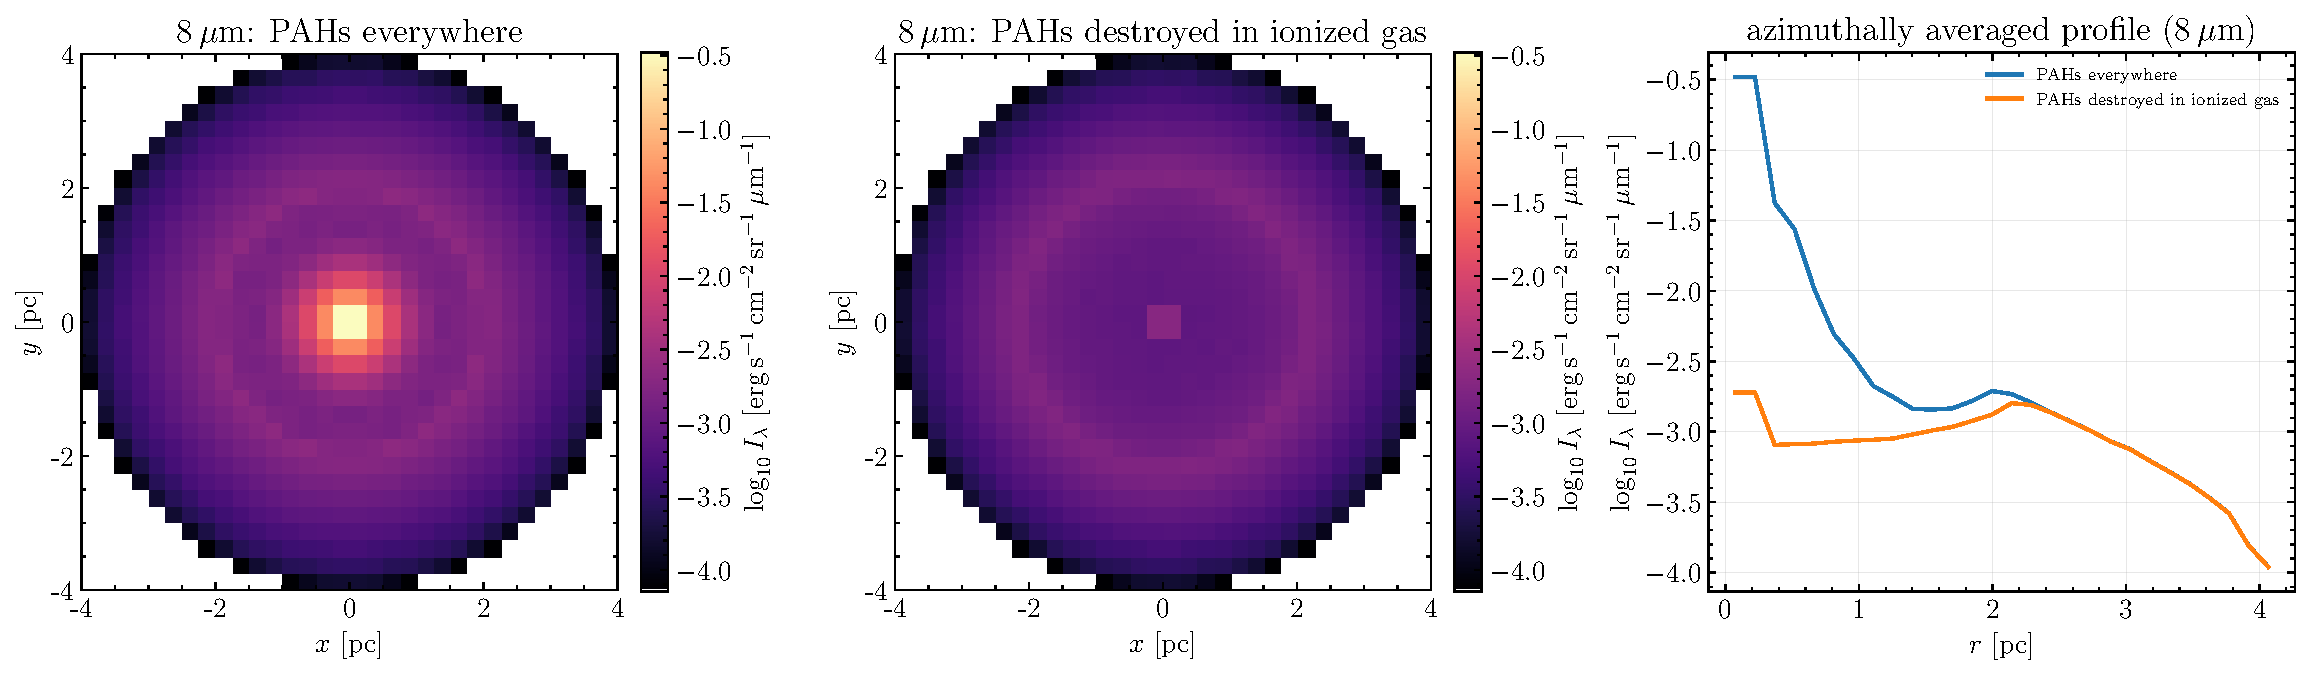
\includegraphics[width=0.95\textwidth]{figures/pahlive_maps.pdf}
% source: figures/make_dust_maps.py, from
%   tests/d_dusty/dustemis_smoke_dustemis.h5 (PAHs everywhere) and
%   tests/d_dusty/pahlive_smoke_dustemis.h5 (live PAH survival).
\caption{Stochastic dust emission at 8\,$\mu$m with the
ionization-dependent PAH share.  The first two panels are two-dimensional
projection maps sharing one brightness scale: the band emissivity, which
\MoCHII{} writes as the power radiated per unit volume and per unit
wavelength into $4\pi$~sr, integrated along the line of sight and divided by
$4\pi$, so the panels show the specific intensity $I_\lambda$ of an
infrared-thin nebula.  Left: PAHs surviving
everywhere, giving a centrally peaked image.  Middle: PAHs destroyed in the
ionized interior ($x_{\mathrm{HII}}$-weighted survival).  Right: the
azimuthally averaged radial profiles of both maps.  Destroying the PAHs
removes the central peak and leaves a broad limb-brightened annulus just
inside the ionization front at $r \simeq 2.1$~pc, visible in the profile as
a local maximum a factor 1.9 above the depressed interior.}
\label{fig:pah}
\end{figure*}

\begin{figure*}[t]
\centering
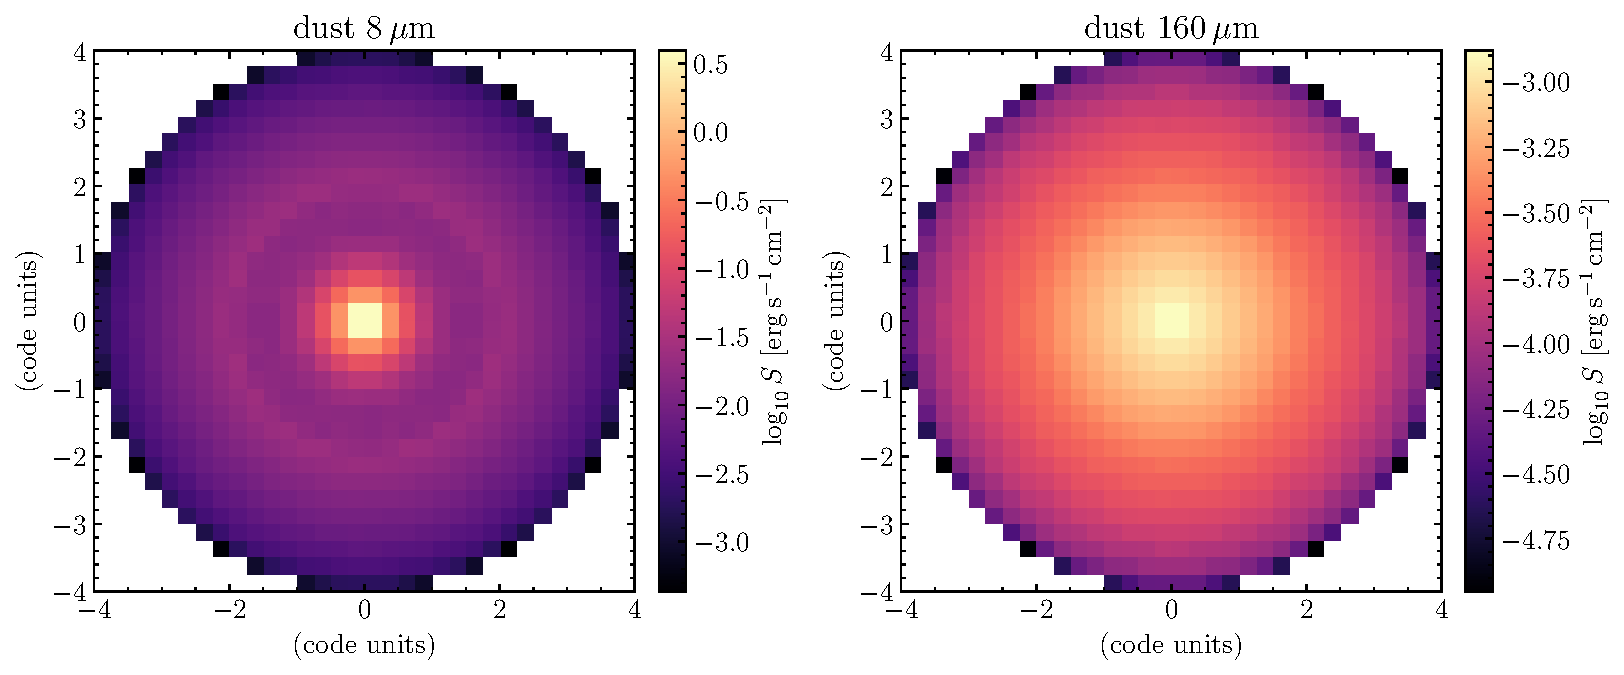
\includegraphics[width=0.95\textwidth]{figures/dustemis_maps.pdf}
% source: figures/make_dust_maps.py, from
%   tests/d_dusty/dustemis_smoke_dustemis.h5.
\caption{Dust emission at 8 and 160\,$\mu$m from the stochastic SEDust
solve, as two-dimensional projection maps of the specific intensity
$I_\lambda$ (left, middle) with their azimuthally averaged radial profiles
(right).  The band emissivity is written as the power radiated per unit
volume and per unit wavelength into $4\pi$~sr, so $I_\lambda$ is that
emissivity integrated along the line of sight and divided by $4\pi$.  The
short
wavelength is centrally peaked (warm inner dust), falling by 3.5~dex across
the sphere, while the far-infrared profile is far flatter (1.6~dex), the
projected signature of the dust temperature gradient.}
\label{fig:dustemis}
\end{figure*}

%==========================================================================
\section{The photodissociation-region skin}
\label{sec:pdr}

With the FUV band extension and three optional switches (all off by
default), \MoCHII{} models the atomic photodissociation-region (PDR) skin
just outside the ionization front.  The switches feed the metal-cascade
electrons into the $\nelec$ closure, add metal photoheating to the thermal
balance, and add grain photoelectric heating and grain recombination
cooling with the \citet{bakes1994} fits driven by the local FUV field
$G_0$, together with the H-impact fine-structure cooling of
[C\,\textsc{ii}] 158\,$\mu$m and [O\,\textsc{i}] 63\,$\mu$m
\citep{barinovs2005}.  The last is essential: the standard cooling fits are
electron-impact only, and with $n_{\mathrm{HI}}/\nelec \sim 10^3$--$10^4$ in
the PDR the hydrogen collisions are the coolant.  Two guards keep the
photoelectric heating physical (evaluated at $\min(T, 10^4\,\mathrm{K})$ so
the fits stay in range, and weighted by $\xHI$ so ionized gas, whose grains
are EUV-charged and whose energy is already routed to the IR, is not
overheated).  Both are necessary: without them the fits are evaluated
outside their validity range and the zone runs away to a false
12--35~kK.

Figure~\ref{fig:pdr} shows the converged radial structure of a PDR test
(a $\nH = 100$ octree sphere with a central source and all three switches
on).  The interior is fully ionized with a sharp front; beyond the front,
the C\,\textsc{ii} fraction is unity, the electron density falls to the
carbon-dominated value $\nelec \simeq A_{\mathrm{C}}\nH$, and the electron
temperature settles to a genuine PDR equilibrium (a $\sim$340~K to
$\sim$208~K gradient, not pinned at the temperature floor).  This is the
atomic PDR skin only: there is no H$_2$/CO chemistry or line transfer, so
the PDR temperatures are first-order estimates, adequate for the ion
structure and rough [C\,\textsc{ii}] emissivities.

\begin{figure}[t]
\centering
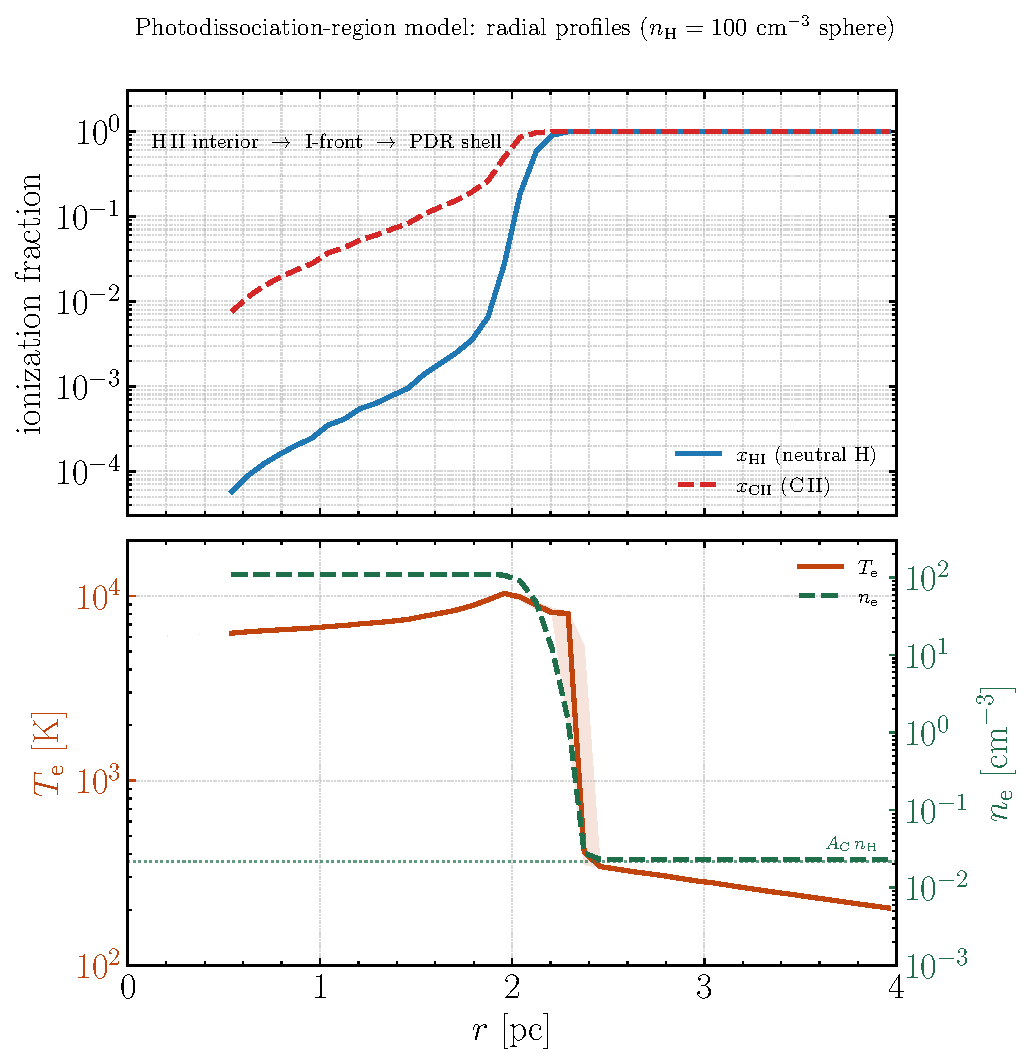
\includegraphics[width=\columnwidth]{figures/pdr_profiles.pdf}
% source: generated by figures/make_pdr_profiles.py from tests/pdr/pdr_L5_rates.h5
\caption{Radial structure of the PDR test: the neutral fraction, electron
temperature, and electron density as a function of radius.  Inside the
front the gas is fully ionized; beyond it the electron density drops to the
carbon-dominated value and the temperature settles to a PDR equilibrium
above the floor.}
\label{fig:pdr}
\end{figure}

%==========================================================================
\section{Summary and outlook}
\label{sec:summary}

\MoCHII{} is a three-dimensional Monte Carlo photoionization code for dusty
nebulae on adaptive octree grids, built by adding a self-consistent
gas-physics layer to a validated dust radiative-transfer engine.  Its
design choices --- octree AMR with solution-driven front refinement, a
zero-variance analytic direct-field estimator with a dedicated Cartesian
DDA backend, an explicit optional Monte Carlo diffuse field, a
data-driven trace-metal registry with modern atomic data, first-class dust
absorption/scattering and equilibrium/stochastic emission with PAH physics,
and peel-off synthetic imaging --- distinguish it from the uniform-grid and
1D codes.  It reproduces analytic attenuation to $+0.08\%$, the Str\"omgren
sphere to $+0.68\%$, and a thermal H/He nebula to $0.77\%$.  On the
Lexington 2000 \HII{} region benchmarks, with continuously sampled Planck
photon energies and cross sections evaluated at each sampled energy, and
with line cooling taken from the level populations at the local electron
density, the
$n_{\mathrm{p}}n_{\mathrm{e}}$-weighted temperature is 8169~K at HII40 and
6925~K at HII20, matching the \textsc{Cloudy} c25.00 solution of the same
two models (8210 and 6910~K) to $0.5\%$ and $0.2\%$; both models are
radiation-bounded, so both outer radii are predicted, and
$L(\mathrm{H}\beta)$ follows the recombination budget to within $8\%$.  The
line-cooling data are checked independently of the temperature by evaluating
the \MoCHII{} cooling terms on a fixed state taken from a \textsc{Cloudy}
c25.00 cooling decomposition: channel by channel the two compilations agree,
and the summed line cooling agrees to $1\%$.  The zero-density limit of the
same cooling data, retained as an option, overestimates the far-infrared
line cooling by $12\%$ at $\nelec = 110\,\mathrm{cm^{-3}}$ and places both
benchmarks $4$--$8\%$ cooler (7894 and 6376~K, inside and just under the
published ranges); the density suppression that removes it is the default.
The \textsc{Cloudy} c25.00 column provides a uniform reference for both
tables and has the same S\,\textsc{ii}/S\,\textsc{iii} ordering as
\MoCHII{}.
The solution-driven
re-refinement reproduces a native high-resolution grid to $+0.008\%$ with
$4.5\times$ fewer cells, the dust coupling closes energy exactly and
reproduces the limb-brightened Spitzer/JWST PAH morphology, and the
atomic PDR skin
recovers the carbon-dominated electron density and a physical PDR
temperature.

Development is ongoing along several lines.  A plane-parallel
(xy-periodic slab) illumination mode with an emergent $I(\mu)$ boundary
tally extends the code to slab and grazing-illumination
geometries.  A He\,\textsc{i} $2^3$S metastable diagnostic supports
synthetic 10833~\AA\ absorption modeling.  A hard-spectrum extension for
planetary nebulae and active galactic nuclei --- higher photon energies,
extended ion stages, and inner-shell/Auger processes --- is planned; the
density-suppressed cooling introduced here already covers the high electron
densities of planetary nebulae.  The trace-metal registry makes further
ions a data operation as the science requires them.  Together these make
\MoCHII{} a tool for modern three-dimensional synthetic observations of
\HII{} regions, planetary nebulae, and the illuminated interstellar and
circumgalactic medium.

\begin{acknowledgments}
K.-I.\ Seon was supported by the Korea Astronomy and Space Science
Institute under the R\&D program (Project No.\ 2026-1-831-02) supervised by
the Korea AeroSpace Administration.
% TODO: acknowledgments -- the MOCASSIN, CHIANTI, Cloudy, PyNeb, and
% Illustris-TNG teams for public data and comparison references, and
% computing resources.
\end{acknowledgments}

\software{MoCHII (\url{https://github.com/seoncafe/MoCHII}),
          MoCafe (\url{https://github.com/seoncafe/MoCafe}),
          CHIANTI \citep{dere1997,delzanna_chianti},
          MOCASSIN \citep{ercolano2003},
          Cloudy \citep{cloudy2023},
          astropy,
          matplotlib,
          NumPy}
% TODO: add astropy/matplotlib/numpy citations if desired, and PyNeb.

\appendix

\section{Fitted atomic-data coefficients}
\label{app:atomic}

The atomic data are fitted offline and evaluated online
(Section~\ref{sec:cooldata}).  Table~\ref{tab:tier1err} gives the quality of
the line-cooling fits of every ion and Table~\ref{tab:tier2} summarizes the
$n$-level diagnostic models; it is generated mechanically from the data
files by \code{paper/tables/make\_atomic\_tables.py}.  The coefficients
themselves --- the amplitudes and excitation temperatures of the
line-cooling fits, and the Burgess--Tully Chebyshev $\Upsilon(T)$ sets of
the $n$-level models, several for each transition --- are distributed with
the code rather than reproduced here.\footnote{The fitted line-cooling
coefficients of every ion are provided as text in
\code{data/atomic/cooling\_fit\_parameters.txt} (and, one file for each ion,
in \code{data/atomic/cooling\_<ion>.txt}), with the fit form, units, fit
range, and maximum fit error documented in \code{data/atomic/README.md};
the $n$-level models are in \code{data/atomic/nlevel\_<ion>.txt}.  Every
file carries a provenance header.}

\clearpage
% Auto-generated by paper/tables/make_atomic_tables.py -- do not edit by hand.
\begin{deluxetable}{lcccclccc}
\tablecaption{Quality of the collisional line-cooling fits: the number of exponential terms $N$, the maximum fit error of each ion over the full $10^3$--$10^5$~K range, and the maximum error restricted to the temperatures that carry the cooling ($\Lambda > 10^{-3}\Lambda_{\max}$).  The two agree for most ions; where they differ, the large full-range error sits in a temperature tail in which the ion radiates negligibly.  The fitted coefficients themselves are distributed with the code (Appendix~\ref{app:atomic}).\label{tab:tier1err}}
\tablehead{\colhead{Ion} & \colhead{$N$} & \colhead{max err} & \colhead{where it cools} & \colhead{} & \colhead{Ion} & \colhead{$N$} & \colhead{max err} & \colhead{where it cools}}
\startdata
H\,\textsc{i} & 4 & 0.52\% & 0.52\% &  & S\,\textsc{iv} & 3 & 0.61\% & 0.61\% \\
C\,\textsc{i} & 6 & 0.27\% & 0.27\% &  & Ar\,\textsc{iii} & 2 & 3.90\% & 3.90\% \\
C\,\textsc{ii} & 5 & 0.35\% & 0.35\% &  & Ar\,\textsc{iv} & 4 & 0.27\% & 0.27\% \\
C\,\textsc{iii} & 6 & 5.48\% & 0.50\% &  & Mg\,\textsc{ii} & 4 & 0.22\% & 0.12\% \\
N\,\textsc{i} & 5 & 0.58\% & 0.34\% &  & Fe\,\textsc{ii} & 5 & 0.56\% & 0.56\% \\
N\,\textsc{ii} & 5 & 0.66\% & 0.66\% &  & Fe\,\textsc{iii} & 5 & 0.48\% & 0.48\% \\
N\,\textsc{iii} & 5 & 0.70\% & 0.70\% &  & Si\,\textsc{ii} & 6 & 0.91\% & 0.91\% \\
O\,\textsc{i} & 6 & 0.20\% & 0.20\% &  & Si\,\textsc{iii} & 6 & 27.70\% & 11.29\% \\
O\,\textsc{ii} & 4 & 0.27\% & 0.15\% &  & Si\,\textsc{iv} & 2 & 0.90\% & 0.90\% \\
O\,\textsc{iii} & 5 & 0.32\% & 0.32\% &  & Cl\,\textsc{ii} & 3 & 8.05\% & 8.05\% \\
Ne\,\textsc{ii} & 5 & 0.40\% & 0.40\% &  & Cl\,\textsc{iii} & 6 & 9.15\% & 9.15\% \\
Ne\,\textsc{iii} & 5 & 0.34\% & 0.34\% &  & Cl\,\textsc{iv} & 2 & 7.30\% & 7.30\% \\
S\,\textsc{ii} & 3 & 2.23\% & 2.16\% &  & Ca\,\textsc{ii} & 4 & 1.03\% & 0.42\% \\
S\,\textsc{iii} & 5 & 0.23\% & 0.23\% &  & Ca\,\textsc{v} & 2 & 4.34\% & 4.34\% \\
\enddata
\end{deluxetable}


% Auto-generated by paper/tables/make_atomic_tables.py -- do not edit by hand.
\providecommand{\rhead}[1]{\multicolumn{1}{r}{\vrule depth 6pt height 12pt width 0pt #1}}
\providecommand{\lhead}[1]{\multicolumn{1}{l}{\vrule depth 6pt height 12pt width 0pt #1}}
\startlongtable
\begin{deluxetable*}{lcccclccc}
\tablecaption{$n$-level diagnostic models: number of levels, number of fitted effective-collision-strength transitions, and the worst transition fit error.  The level energies and radiative $A$-values are from CHIANTI v11.0.2, and $\Upsilon(T)$ is a low-order Chebyshev fit in Burgess--Tully scaled space over $10^3$--$10^5$~K; the full coefficient sets are in the provenance-headed files \texttt{data/atomic/nlevel\_<ion>.txt}.\label{tab:tier2}}
\tablehead{\colhead{Ion} & \colhead{levels} & \colhead{transitions} & \colhead{worst err} & \colhead{} & \colhead{Ion} & \colhead{levels} & \colhead{transitions} & \colhead{worst err}}
\startdata
H\,\textsc{i} & 25 & 45 & 0.20\% &  & S\,\textsc{iv} & 5 & 10 & 0.18\% \\
C\,\textsc{i} & 5 & 10 & 0.52\% &  & Ar\,\textsc{iii} & 5 & 10 & 0.19\% \\
C\,\textsc{ii} & 5 & 10 & 0.56\% &  & Ar\,\textsc{iv} & 5 & 10 & 0.20\% \\
C\,\textsc{iii} & 5 & 10 & 0.35\% &  & Mg\,\textsc{ii} & 3 & 3 & 0.15\% \\
N\,\textsc{i} & 5 & 10 & 0.78\% &  & Fe\,\textsc{ii} & 13 & 78 & 0.20\% \\
N\,\textsc{ii} & 5 & 10 & 0.17\% &  & Fe\,\textsc{iii} & 14 & 91 & 0.20\% \\
N\,\textsc{iii} & 5 & 10 & 0.45\% &  & Si\,\textsc{ii} & 5 & 10 & 0.19\% \\
O\,\textsc{i} & 5 & 10 & 0.17\% &  & Si\,\textsc{iii} & 5 & 10 & 0.65\% \\
O\,\textsc{ii} & 5 & 10 & 0.27\% &  & Si\,\textsc{iv} & 3 & 3 & 0.54\% \\
O\,\textsc{iii} & 6 & 15 & 1.68\% &  & Cl\,\textsc{ii} & 5 & 10 & 0.17\% \\
Ne\,\textsc{ii} & 2 & 1 & 0.16\% &  & Cl\,\textsc{iii} & 5 & 10 & 0.19\% \\
Ne\,\textsc{iii} & 5 & 10 & 0.19\% &  & Cl\,\textsc{iv} & 5 & 10 & 0.19\% \\
S\,\textsc{ii} & 5 & 10 & 1.25\% &  & Ca\,\textsc{ii} & 5 & 10 & 0.19\% \\
S\,\textsc{iii} & 6 & 15 & 0.29\% &  & Ca\,\textsc{v} & 5 & 10 & 0.19\% \\
\enddata
\tablecomments{Expanded 16/34-level Fe\,\textsc{ii}/\textsc{iii} models (\texttt{nlevel\_fe\_\{2,3\}\_full.txt}) are available for iron-line studies.  Ar\,\textsc{ii}, Cl\,\textsc{v}, and Ca\,\textsc{iii}/\textsc{iv} have no CHIANTI~v11 level data and are tracked in the ionization balance without lines.}
\end{deluxetable*}


\section{Full Lexington benchmark line lists}
\label{app:lines}

\begin{figure*}[t]
\centering
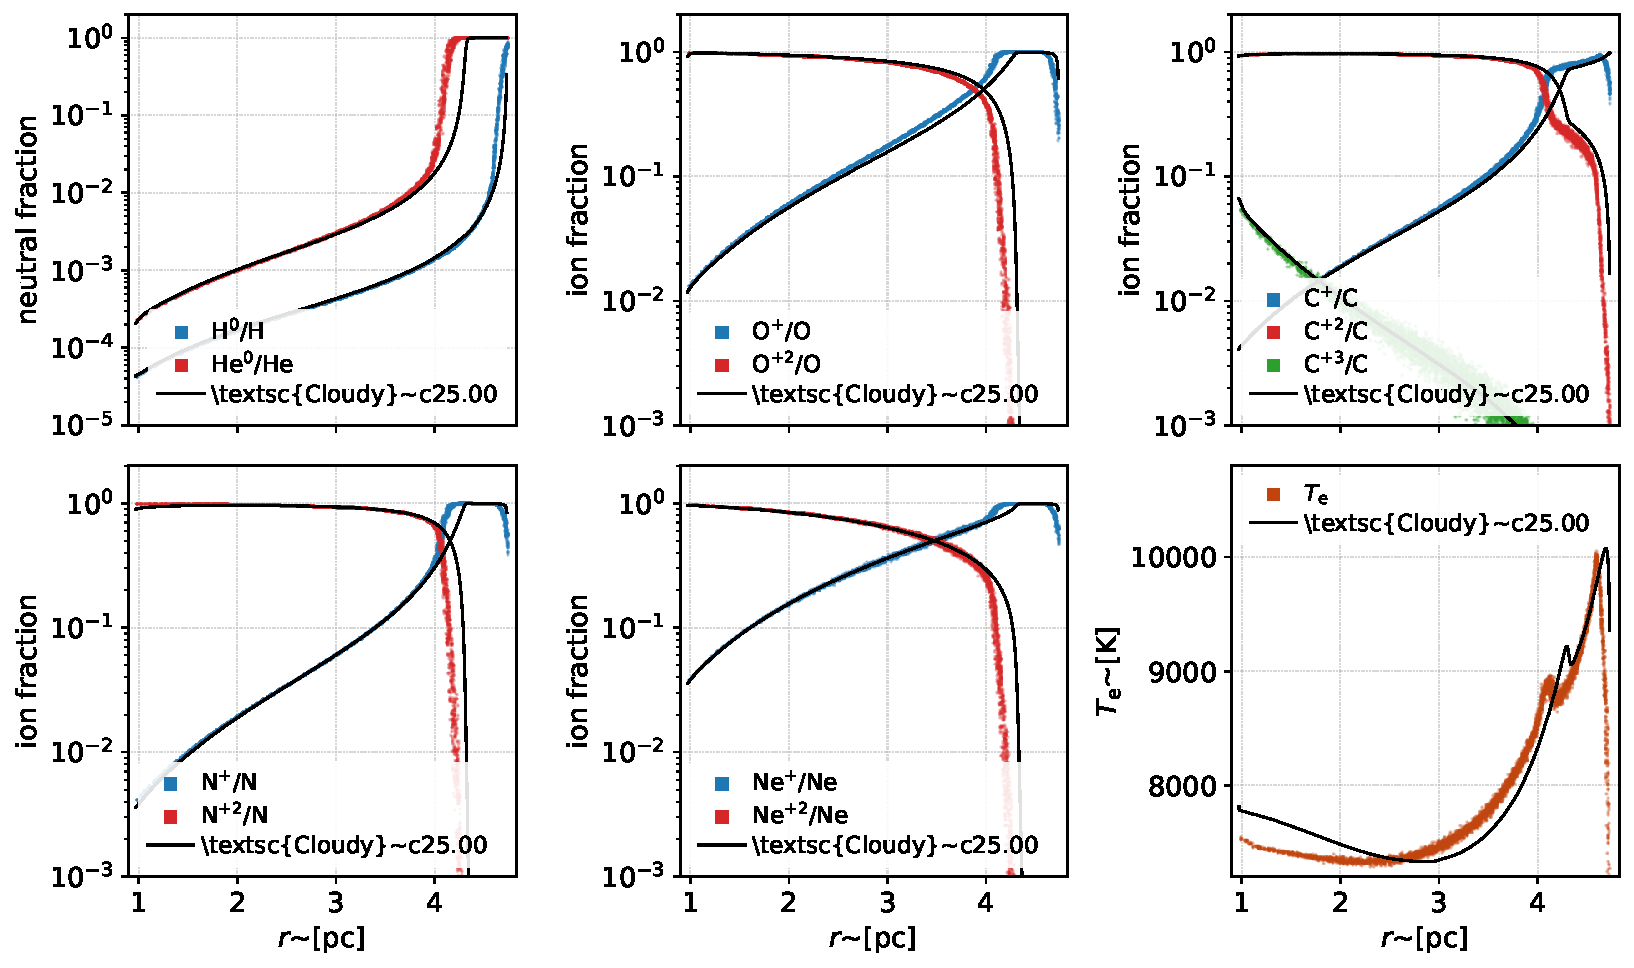
\includegraphics[width=\textwidth]{figures/wood_hii40.pdf}
% source: results/continuous_energy/production/hii40_continuous_rates.h5
% and the Cloudy c25.00 save files
% tests/cloudy_c25/hii40_c25.{ovr,ele_h,ele_he,ele_c,ele_n,ele_o,ele_ne},
% via paper/python/make_wood_benchmark.py
\caption{Lexington HII40 benchmark: radial ionization and temperature
structure of the \MoCHII{} solution, in the panel layout of
\citet{wood2004}, their Figure 1.  Each point is one octree leaf inside the
prescribed shell, thinned at random for legibility; the temperature panel
shows the leaves that are less than 95\% neutral, the convention of
\citet{wood2004}.  Nitrogen stops at N$^{+2}$ because the registry carries
three nitrogen stages for this model.  This is the same run as the
\MoCHII{} column of Table~\ref{tab:wood40}, with continuous Planck-sampled
stellar photon energies and cross sections evaluated at the sampled energy;
the 32-bin radiation array is diagnostic only.  Black lines are
\textsc{Cloudy}~c25.00 on the same
model --- the run behind the C25 column of Table~\ref{tab:wood40}, whose
input is the unmodified c25.00 test-suite deck
\code{tsuite/auto/hii\_paris.in} --- drawn as a line as
\citet{wood2004} draw \textsc{Cloudy} in their own figures.  The
\textsc{Cloudy} profile is cut at the outer radius of the \MoCHII{} shell so
that both codes cover one volume, and the 95\% cut is applied to its zones
as well.  In the temperature panel the \MoCHII{} points run below the
\textsc{Cloudy} curve through the interior and cross it at the front.}
\label{fig:wood40}
\end{figure*}

\begin{figure*}[t]
\centering
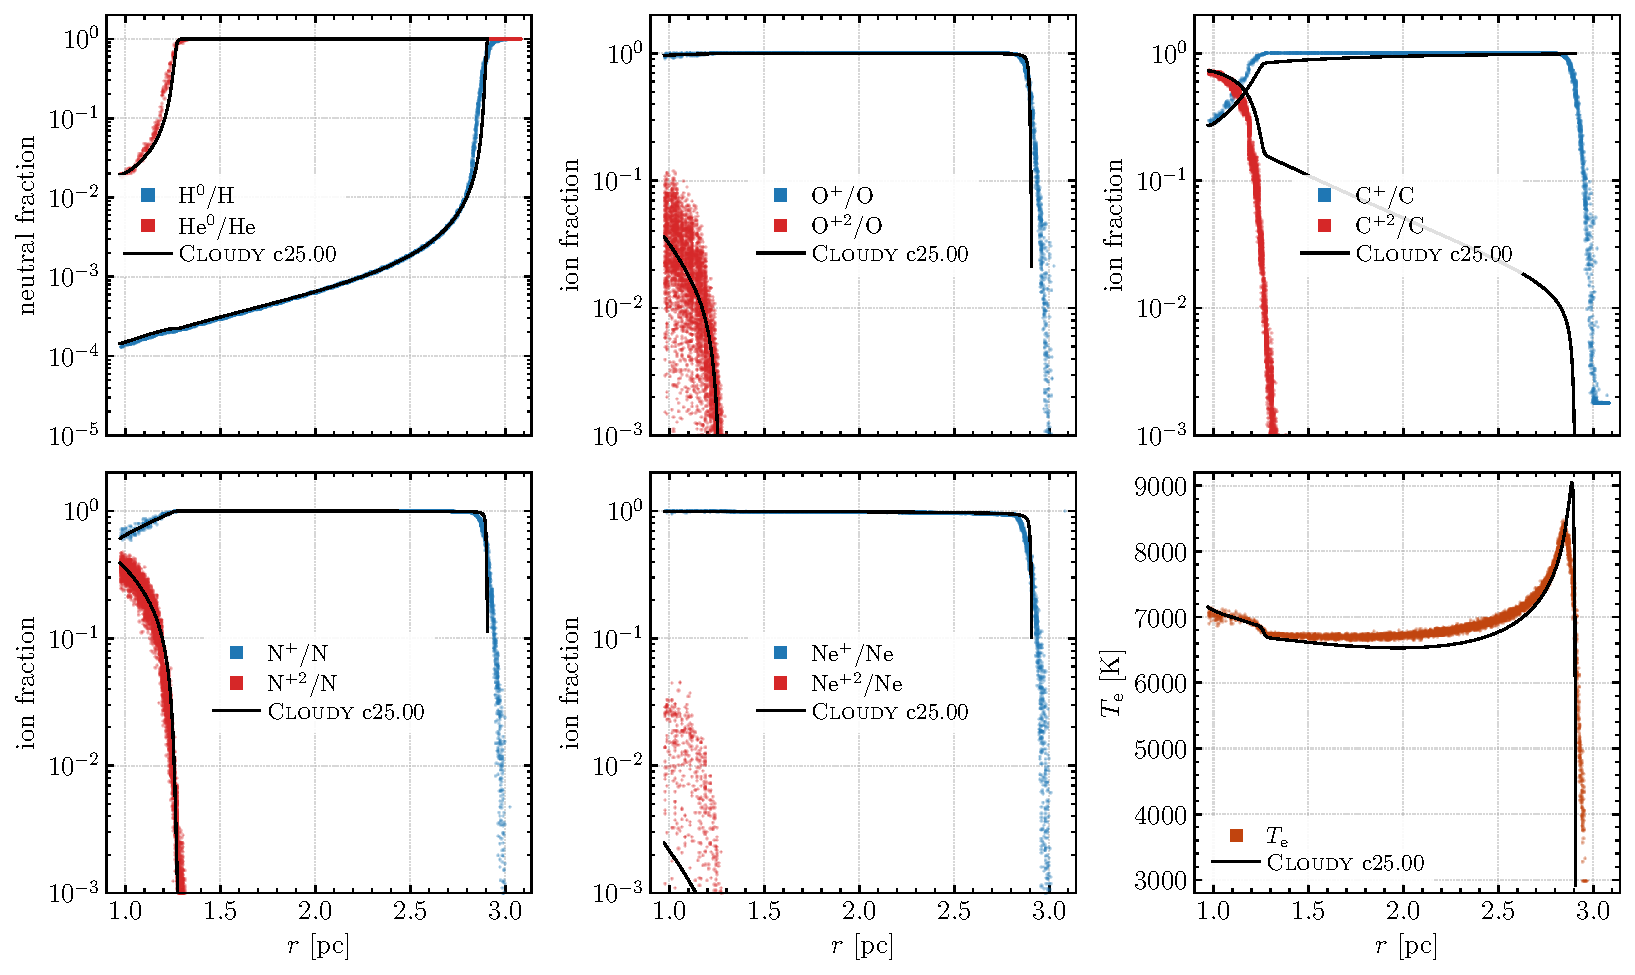
\includegraphics[width=\textwidth]{figures/wood_hii20.pdf}
% source: results/continuous_energy/production/hii20_continuous_rates.h5
% and the Cloudy c25.00 save files
% tests/cloudy_c25/hii20_c25.{ovr,ele_h,ele_he,ele_c,ele_n,ele_o,ele_ne},
% via paper/python/make_wood_benchmark.py
\caption{Lexington HII20 benchmark, in the panel layout of
\citet{wood2004}, their Figure 2; conventions as in
Figure~\ref{fig:wood40}.  Ne$^{+2}$ is confined within 1.4~pc, and
C$^{+3}$ stays below the plotted range and carries no series.  This is the
same run as the \MoCHII{} column of Table~\ref{tab:wood20}.  At 20~kK the
helium-ionizing photons are so few that helium is neutral beyond 1.4~pc.
The continuous-energy treatment nonetheless preserves the weak C$^{+2}$
tail outside that helium transition.  Black lines are \textsc{Cloudy}~c25.00
on the same model, from the
unmodified c25.00 deck \code{tsuite/auto/hii\_coolstar.in} behind the C25
column of Table~\ref{tab:wood20}.  \textsc{Cloudy} stops on its own
criterion at 2.91~pc, short of the outer radius of the \MoCHII{} shell, so
its curves end there, and its final near-vertical fall is the recombination
front itself, resolved in zones far finer than a \MoCHII{} cell.}
\label{fig:wood20}
\end{figure*}

Tables~\ref{tab:wood40} and~\ref{tab:wood20} give the complete Lexington
HII40 and HII20 benchmark line lists discussed in Section~\ref{sec:hii}, in
the form used by \citet{wood2004}: the eight published codes of the
\citet{ercolano2003} compilation, the \citet{wood2004} Monte Carlo code
(WME), a \textsc{Cloudy}~c25.00 calculation (C25), and the \MoCHII{} column.
Line intensities are relative to H$\beta$.

% Tables tab:wood40 / tab:wood20: generated by tables/make_wood_tables.py.
% Published columns transcribed from the LaTeX source of Wood et al. (2004)
% (arXiv:astro-ph/0311584, kwood.tex) and checked cell by cell against it;
% the MoCHII column is computed from the continuous-energy production lines
% in results/continuous_energy/production/.
\clearpage
%% Generated by tables/make_wood_tables.py -- do not edit.
\begin{deluxetable*}{lccccccccccc}
\tablecaption{Lexington \HII{} region benchmark HII40 (40~kK blackbody):
the published multi-code results of \citet[][their Table 1]{wood2004}, with a
\textsc{Cloudy} c25.00 calculation and the \MoCHII{} result appended.  Line
intensities are relative to H$\beta$.\label{tab:wood40}}
\tablewidth{0pt}
\tabletypesize{\footnotesize}
\tablehead{\colhead{Quantity} & \colhead{GF} & \colhead{C25} & \colhead{HN} & \colhead{DP} & \colhead{TK} & \colhead{PH} & \colhead{RS} & \colhead{RR} & \colhead{BE} & \colhead{WME} & \colhead{\MoCHII{}}}
\startdata
$L(\mathrm{H}\beta)/10^{37}\,\mathrm{erg\,s^{-1}}$ & 2.06 & 2.06 & 2.02 & 2.02 & 2.10 & 2.05 & 2.07 & 2.05 & 2.02 & 2.01 & 1.94 \\
\HeI{} 5876 & 0.119 & 0.100 & 0.112 & 0.113 & 0.116 & 0.118 & 0.116 & \nodata & 0.114 & 0.114 & 0.106 \\
C\,\textsc{ii}] 2325+ & 0.157 & 0.189 & 0.141 & 0.139 & 0.110 & 0.166 & 0.096 & 0.178 & 0.148 & 0.172 & 0.174 \\
C\,\textsc{iii}] 1907+1909 & 0.071 & 0.062 & 0.076 & 0.069 & 0.091 & 0.060 & 0.066 & 0.074 & 0.041 & 0.078 & 0.057 \\
$[$N\,\textsc{ii}$]$ 122\,$\mu$m & 0.027 & 0.030 & 0.037 & 0.034 & \nodata & 0.032 & 0.035 & 0.030 & 0.036 & 0.031 & 0.032 \\
$[$N\,\textsc{ii}$]$ 6584+6548 & 0.669 & 0.669 & 0.817 & 0.725 & 0.69 & 0.736 & 0.723 & 0.807 & 0.852 & 0.742 & 0.702 \\
$[$N\,\textsc{ii}$]$ 5755 & 0.0050 & 0.0060 & 0.0054 & 0.0050 & \nodata & 0.0064 & 0.0050 & 0.0068 & 0.0061 & 0.0057 & 0.0060 \\
$[$N\,\textsc{iii}$]$ 57.3\,$\mu$m & 0.306 & 0.286 & 0.261 & 0.311 & \nodata & 0.292 & 0.273 & 0.301 & 0.223 & 0.308 & 0.288 \\
$[$O\,\textsc{i}$]$ 6300+6363 & 0.0094 & 0.0112 & 0.0086 & 0.0088 & 0.012 & 0.0059 & 0.0070 & \nodata & 0.0065 & 0.011 & 0.0170 \\
$[$O\,\textsc{ii}$]$ 7320+7330 & 0.029 & 0.033 & 0.030 & 0.031 & 0.023 & 0.032 & 0.024 & 0.036 & 0.025 & 0.033 & 0.035 \\
$[$O\,\textsc{ii}$]$ 3726+3729 & 1.94 & 2.32 & 2.17 & 2.12 & 1.6 & 2.19 & 1.88 & 2.26 & 1.92 & 2.23 & 2.32 \\
$[$O\,\textsc{iii}$]$ 52+88\,$\mu$m & 2.35 & 2.40 & 2.10 & 2.26 & 2.17 & 2.34 & 2.29 & 2.34 & 2.28 & 2.42 & 2.43 \\
$[$O\,\textsc{iii}$]$ 5007+4959 & 2.21 & 2.46 & 2.38 & 2.20 & 3.27 & 1.93 & 2.17 & 2.08 & 1.64 & 2.34 & 2.37 \\
$[$O\,\textsc{iii}$]$ 4363 & 0.00235 & 0.0046 & 0.0046 & 0.0041 & 0.0070 & 0.0032 & 0.0040 & 0.0035 & 0.0022 & 0.0044 & 0.0044 \\
$[$Ne\,\textsc{ii}$]$ 12.8\,$\mu$m & 0.177 & 0.200 & 0.195 & 0.192 & \nodata & 0.181 & 0.217 & 0.196 & 0.212 & 0.192 & 0.206 \\
$[$Ne\,\textsc{iii}$]$ 15.5\,$\mu$m & 0.294 & 0.216 & 0.264 & 0.270 & 0.35 & 0.429 & 0.350 & 0.417 & 0.267 & 0.263 & 0.284 \\
$[$Ne\,\textsc{iii}$]$ 3869+3968 & 0.084 & 0.058 & 0.087 & 0.071 & 0.092 & 0.087 & 0.083 & 0.086 & 0.053 & 0.063 & 0.072 \\
$[$S\,\textsc{ii}$]$ 6716+6731 & 0.137 & 0.304 & 0.166 & 0.153 & 0.315 & 0.155 & 0.133 & 0.130 & 0.141 & 0.18 & 0.323 \\
$[$S\,\textsc{ii}$]$ 4068+4076 & 0.0093 & 0.0142 & 0.0090 & 0.0100 & 0.026 & 0.0070 & 0.005 & 0.0060 & 0.0060 & 0.0094 & 0.0140 \\
$[$S\,\textsc{iii}$]$ 18.7\,$\mu$m & 0.627 & 0.504 & 0.750 & 0.726 & 0.535 & 0.556 & 0.567 & 0.580 & 0.574 & 0.623 & 0.509 \\
$[$S\,\textsc{iii}$]$ 9532+9069 & 1.13 & 1.00 & 1.19 & 1.16 & 1.25 & 1.23 & 1.25 & 1.28 & 1.21 & 1.44 & 1.01 \\
$10^{3}\times\Delta(\mathrm{BC}\,3645)$/\AA & 4.88 & \nodata & \nodata & 4.95 & \nodata & 5.00 & 5.70 & \nodata & 5.47 & 4.96 & \nodata \\
$T_{\mathrm{inner}}$ / K & 7719 & 7812 & 7668 & 7663 & 8318 & 7440 & 7644 & 7399 & 7370 & 7743 & 7540 \\
$\langle T[N_{\mathrm{p}}N_{\mathrm{e}}]\rangle$ / K & 7940 & 8210 & 7936 & 8082 & 8199 & 8030 & 8022 & 8060 & 7720 & 8183 & 8202 \\
$R_{\mathrm{out}}/10^{19}$\,cm & 1.46 & 1.47 & 1.46 & 1.46 & 1.45 & 1.46 & 1.47 & 1.46 & 1.46 & 1.45 & 1.45 \\
$\langle\mathrm{He^{+}}\rangle/\langle\mathrm{H^{+}}\rangle$ & 0.787 & 0.741 & 0.727 & 0.754 & 0.77 & 0.764 & 0.804 & 0.829 & 0.715 & 0.771 & 0.704 \\
\enddata
\tablecomments{Codes, in the notation of \citet{wood2004}: GF =
Ferland's \textsc{Cloudy}; HN = Netzer's \textsc{Ion}; DP = P\'equignot's
\textsc{Nebu}; TK = Kallman's \textsc{XStar}; PH = Harrington's code;
RS = Sutherland's \textsc{Mappings}; RR = Rubin's \textsc{Nebula};
BE = Ercolano's \textsc{Mocassin}; WME = the code of \citet{wood2004}
itself.  Columns GF--BE agree entry by entry with Tables 4 and 5 of
\citet{ercolano2003}, the compilation of the published columns.
C25 is \textsc{Cloudy} c25.00 \citep{cloudy2025} run for this paper and
provides a uniform one-dimensional reference alongside the published
multi-code spread.
Its physics input is the unmodified c25.00 test-suite file
\code{tsuite/auto/hii\_paris.in} (HII40) or \code{hii\_coolstar.in} (HII20)
--- \textsc{Cloudy}'s own maintained version of these benchmarks --- with
only output commands appended; line luminosities come from a \code{save line
list absolute} file and are divided by the \textsc{Cloudy} H\,\textsc{i}
4861.32\,\AA{} luminosity, and the \textsc{Cloudy} blends summed for each row
are listed in \code{tables/make\_wood\_tables.py}.  Unlike the published
columns, C25 runs to the stopping criterion of its own deck rather than to a
prescribed outer radius --- an electron fraction of $10^{-2}$ at HII40, the
1000~K temperature floor at HII20 --- which mainly affects the
low-ionization rows fed by the partly neutral edge.
The \MoCHII{} column uses continuous stellar photon energies sampled from
the Planck spectrum with a Sobol sequence (seed 20260728), and evaluates
photoionization cross sections at each sampled energy; the 32-bin ionizing
array is a diagnostic tally only.  It uses the explicit Monte Carlo diffuse
field including the \HeI{} channels (case~A, matching the transfer treatment
of the published codes), and Badnell 2023 recombination with the Mao \&
Kaastra 2016 ground-level split, at $2^{25}$ stellar packets with the
volume-integrated convergence criterion; the ionizing luminosity is set from
the benchmark $L({\rm BB})$ so that $Q({\rm H})$ matches the specification;
blends are the sum of the
\MoCHII{} components listed in \code{tables/make\_wood\_tables.py}, and
\MoCHII{} wavelengths are vacuum values.  The \MoCHII{} structural entries
are computed from the same run: $T_{\mathrm{inner}}$ is the mean $\Te$ of the
cells at the illuminated inner edge, $R_{\mathrm{out}}$ the radius at which
the shell-averaged $x_{\mathrm{HII}}$ falls through 0.5, and the helium ratio
follows Eq.~(17) of \citet{ercolano2003},
$\langle\mathrm{He^{+}}\rangle/\langle\mathrm{H^{+}}\rangle =
\int \nelec n(\mathrm{He^{+}})\,{\rm d}V / \int \nelec n_{\mathrm{p}}\,{\rm d}V
\times n_{\mathrm{H}}/n_{\mathrm{He}}$.  Where the ionized gas still fills the
outermost shell of the prescribed sphere, $R_{\mathrm{out}}$ would be set by the
grid rather than predicted, and the entry is left empty.  The Balmer jump is
not computed.  The H$\beta$ row is headed $10^{36}$
erg\,s$^{-1}$ in the published table; the values listed there are the
$10^{37}$~erg\,s$^{-1}$ values of \citet{ercolano2003}, and the heading is
corrected accordingly here.}
\end{deluxetable*}

%% Generated by tables/make_wood_tables.py -- do not edit.
\begin{deluxetable*}{lccccccccccc}
\tablecaption{Lexington \HII{} region benchmark HII20 (20~kK blackbody):
the published multi-code results of \citet[][their Table 2]{wood2004}, with a
current \textsc{Cloudy} c25.00 run and the \MoCHII{} result appended.  Line
intensities are relative to H$\beta$.\label{tab:wood20}}
\tablewidth{0pt}
\tabletypesize{\footnotesize}
\tablehead{\colhead{Quantity} & \colhead{GF} & \colhead{C25} & \colhead{HN} & \colhead{DP} & \colhead{TK} & \colhead{PH} & \colhead{RS} & \colhead{RR} & \colhead{BE} & \colhead{WME} & \colhead{\MoCHII{}}}
\startdata
$L(\mathrm{H}\beta)/10^{36}\,\mathrm{erg\,s^{-1}}$ & 4.85 & 4.99 & 4.85 & 4.83 & 4.90 & 4.93 & 5.04 & 4.89 & 4.97 & 4.87 & 4.71 \\
\HeI{} 5876 & 0.0072 & 0.0061 & 0.008 & 0.0073 & 0.008 & 0.0074 & 0.0110 & \nodata & 0.0069 & 0.00684 & 0.0068 \\
C\,\textsc{ii}] 2325+ & 0.054 & 0.076 & 0.047 & 0.046 & 0.040 & 0.060 & 0.038 & 0.063 & 0.042 & 0.053 & 0.068 \\
$[$N\,\textsc{ii}$]$ 122\,$\mu$m & 0.068 & 0.070 & \nodata & 0.072 & 0.007 & 0.072 & 0.071 & 0.071 & 0.071 & 0.067 & 0.073 \\
$[$N\,\textsc{ii}$]$ 6584+6548 & 0.745 & 0.809 & 0.786 & 0.785 & 0.925 & 0.843 & 0.803 & 0.915 & 0.846 & 0.778 & 0.840 \\
$[$N\,\textsc{ii}$]$ 5755 & 0.0028 & 0.0032 & 0.0024 & 0.0023 & 0.0029 & 0.0033 & 0.0030 & 0.0033 & 0.0025 & 0.0025 & 0.0032 \\
$[$N\,\textsc{iii}$]$ 57.3\,$\mu$m & 0.0040 & 0.0038 & 0.0030 & 0.0032 & 0.0047 & 0.0031 & 0.0020 & 0.0022 & 0.0019 & 0.0049 & 0.0039 \\
$[$O\,\textsc{i}$]$ 6300+6363 & 0.0080 & 0.0084 & 0.0060 & 0.0063 & 0.0059 & 0.0047 & 0.0050 & \nodata & 0.0088 & 0.055 & 0.0112 \\
$[$O\,\textsc{ii}$]$ 7320+7330 & 0.0087 & 0.0113 & 0.0085 & 0.0089 & 0.0037 & 0.0103 & 0.0080 & 0.0100 & 0.0064 & 0.0089 & 0.0122 \\
$[$O\,\textsc{ii}$]$ 3726+3729 & 1.01 & 1.40 & 1.13 & 1.10 & 1.04 & 1.22 & 1.08 & 1.17 & 0.909 & 1.12 & 1.41 \\
$[$O\,\textsc{iii}$]$ 52+88\,$\mu$m & 0.0030 & 0.0033 & 0.0026 & 0.0026 & 0.0040 & 0.0037 & 0.0020 & 0.0017 & 0.0022 & 0.0044 & 0.0033 \\
$[$O\,\textsc{iii}$]$ 5007+4959 & 0.0021 & 0.0023 & 0.0016 & 0.0015 & 0.0024 & 0.0014 & 0.0010 & 0.0010 & 0.0011 & 0.0026 & 0.0021 \\
$[$Ne\,\textsc{ii}$]$ 12.8\,$\mu$m & 0.264 & 0.296 & 0.267 & 0.276 & 0.27 & 0.271 & 0.286 & 0.290 & 0.295 & 0.289 & 0.303 \\
$[$S\,\textsc{ii}$]$ 6716+6731 & 0.499 & 0.744 & 0.473 & 0.459 & 1.02 & 0.555 & 0.435 & 0.492 & 0.486 & 0.521 & 0.778 \\
$[$S\,\textsc{ii}$]$ 4068+4076 & 0.022 & 0.023 & 0.017 & 0.020 & 0.052 & 0.017 & 0.012 & 0.015 & 0.013 & 0.017 & 0.023 \\
$[$S\,\textsc{iii}$]$ 18.7\,$\mu$m & 0.445 & 0.209 & 0.460 & 0.441 & 0.34 & 0.365 & 0.398 & 0.374 & 0.371 & 0.381 & 0.215 \\
$[$S\,\textsc{iii}$]$ 9532+9069 & 0.501 & 0.293 & 0.480 & 0.465 & 0.56 & 0.549 & 0.604 & 0.551 & 0.526 & 0.602 & 0.303 \\
$10^{3}\times\Delta(\mathrm{BC}\,3645)$/\AA & 5.54 & \nodata & \nodata & 5.62 & \nodata & 5.57 & 5.50 & \nodata & 6.18 & 5.52 & \nodata \\
$T_{\mathrm{inner}}$ / K & 7224 & 7155 & 6815 & 6789 & 6607 & 6742 & 6900 & 6708 & 6562 & 6852 & 6938 \\
$\langle T[N_{\mathrm{p}}N_{\mathrm{e}}]\rangle$ / K & 6680 & 6910 & 6650 & 6626 & 6662 & 6749 & 6663 & 6679 & 6402 & 6692 & 6916 \\
$R_{\mathrm{out}}/10^{18}$\,cm & 8.89 & 8.97 & 8.88 & 8.88 & 8.7 & 8.95 & 9.01 & 8.92 & 8.89 & 8.73 & 8.89 \\
$\langle\mathrm{He^{+}}\rangle/\langle\mathrm{H^{+}}\rangle$ & 0.048 & 0.043 & 0.051 & 0.049 & 0.048 & 0.044 & 0.077 & 0.034 & 0.041 & 0.047 & 0.046 \\
\enddata
\tablecomments{Codes, in the notation of \citet{wood2004}: GF =
Ferland's \textsc{Cloudy}; HN = Netzer's \textsc{Ion}; DP = P\'equignot's
\textsc{Nebu}; TK = Kallman's \textsc{XStar}; PH = Harrington's code;
RS = Sutherland's \textsc{Mappings}; RR = Rubin's \textsc{Nebula};
BE = Ercolano's \textsc{Mocassin}; WME = the code of \citet{wood2004}
itself.  Columns GF--BE agree entry by entry with Tables 4 and 5 of
\citet{ercolano2003}, the compilation of the published columns.
C25 is \textsc{Cloudy} c25.00 \citep{cloudy2025} run for this paper, and
is included because the published GF column dates from the 1990s version of
the same code, so the two together measure how far that reference has moved.
Its physics input is the unmodified c25.00 test-suite file
\code{tsuite/auto/hii\_paris.in} (HII40) or \code{hii\_coolstar.in} (HII20)
--- \textsc{Cloudy}'s own maintained version of these benchmarks --- with
only output commands appended; line luminosities come from a \code{save line
list absolute} file and are divided by the \textsc{Cloudy} H\,\textsc{i}
4861.32\,\AA{} luminosity, and the \textsc{Cloudy} blends summed for each row
are listed in \code{tables/make\_wood\_tables.py}.  Unlike the published
columns, C25 runs to the stopping criterion of its own deck rather than to a
prescribed outer radius --- an electron fraction of $10^{-2}$ at HII40, the
1000~K temperature floor at HII20 --- which mainly affects the
low-ionization rows fed by the partly neutral edge.
The \MoCHII{} column uses continuous stellar photon energies sampled from
the Planck spectrum with a Sobol sequence (seed 20260728), and evaluates
photoionization cross sections at each sampled energy; the 32-bin ionizing
array is a diagnostic tally only.  It uses the explicit Monte Carlo diffuse
field including the \HeI{} channels (case~A, matching the transfer treatment
of the published codes), and Badnell 2023 recombination with the Mao \&
Kaastra 2016 ground-level split, at $2^{25}$ stellar packets with the
volume-integrated convergence criterion; the ionizing luminosity is set from
the benchmark $L({\rm BB})$ so that $Q({\rm H})$ matches the specification;
blends are the sum of the
\MoCHII{} components listed in \code{tables/make\_wood\_tables.py}, and
\MoCHII{} wavelengths are vacuum values.  The \MoCHII{} structural entries
are computed from the same run: $T_{\mathrm{inner}}$ is the mean $\Te$ of the
cells at the illuminated inner edge, $R_{\mathrm{out}}$ the radius at which
the shell-averaged $x_{\mathrm{HII}}$ falls through 0.5, and the helium ratio
follows Eq.~(17) of \citet{ercolano2003},
$\langle\mathrm{He^{+}}\rangle/\langle\mathrm{H^{+}}\rangle =
\int \nelec n(\mathrm{He^{+}})\,{\rm d}V / \int \nelec n_{\mathrm{p}}\,{\rm d}V
\times n_{\mathrm{H}}/n_{\mathrm{He}}$.  Where the ionized gas still fills the
outermost shell of the prescribed sphere, $R_{\mathrm{out}}$ would be set by the
grid rather than predicted, and the entry is left empty.  The Balmer jump is
not computed.}
\end{deluxetable*}


\bibliographystyle{aasjournalv7.1}
\bibliography{mochii}

\end{document}
